\documentclass{pnastwo}
\usepackage{cite}
\usepackage{color}
\usepackage{pgf}
%\usepackage{hyperref}
\usepackage[normalem]{ulem}
\newcommand{\jri}[1]{\textcolor{red}{\scriptsize #1}}
\newcommand{\citex}{\textcolor{red}{\bf CITE}}
\newcommand{\X}{\textcolor{red}{\bf X}}
\usepackage{multibib}


\begin{document}


\title{Demography and linked selection in wild and domesticated maize}
\author{Timothy M. Beissinger\affil{1}{Dept. of Plant Sciences, University of
    California, Davis, CA, USA}\affil{2}{US Department of Agriculture, Agricultural Research Service, Columbia, MO, USA}\affil{3}{Division of Plant Sciences, University of Missouri, Columbia, MO, USA} Li Wang\affil{4}{Iowa State University, Ames, IA, USA}, Kate Crosby\affil{1}{}, Arun
  Durvasula\affil{1}{}, Matthew Hufford\affil{4}{}, \and Jeffrey
  Ross-Ibarra\affil{1}{}\affil{5}{Genome Center and Center for population biology, University of
    California, Davis, CA, USA} }

\significancetext{Patterns of linked selection, or the impact of selection on sites that neighbor a functional variant, play a critical role in shaping the genetic diversity of organisms.  In this work, we demonstrate that selection against deleterious mutations leaves a pronounced signature on the maize genome, reducing diversity in and immediately around genes. We show how demography interacts with selection to impact genome-wide patterns of diversity, including the important observation that rapid population expansion can increase the efficiency of selection as much as a sudden population bottleneck can weaken it. Along the way, we develop the first estimate the demographic parameters of the maize domestication from whole genome sequence data. }

\maketitle

\begin{article}

\begin{abstract}
  Unique selective and demographic forces operate on domesticated plant species. These forces interact during and after domestication to generate the patterns of DNA variability that are persistent today. To quantify the interplay between demography and selection, we investigated genetic diversity in maize, one of the most important crops for food, feed, and fuel world-wide. Our sample included whole genome sequence data from 23 maize and 13 teosinte individuals.  We obtained a complete estimate of the population size fluctuations and other demographic parameters experienced by maize as it was domesticated from teosinte. Here, we show that maize went through a domestication bottleneck with a population size of approximately 5\% that of teosinte before it experienced rapid population size expansion post-domestication. We observe that hard sweeps on genic mutations are not the primary force driving maize evolution. We find that a reduced population size during domestication decreased the efficiency of purifying selection to purge deleterious alleles from maize. However, expansion after domestication has since increased the efficiency of purifying selection to levels exceeding those seen in teosinte. Our results demonstrate that particularly in domesticated species or bottlenecked species, demographic and selective history in the ancient and recent past both contribute to genetic variability that is present today, providing substantial implications for the continued improvement of domesticated species.
  
\end{abstract}

\dropcap{D}omesticated plant species evolve in a unique fashion
compared to their wild counterparts \cite{doebley2006}. This
is a result of both the anthropomorphic nature of artificial selection on
domesticates \cite{purugganan2009} as well as the demographic characteristics of the domestication
bottleneck(s) that they tend to have experienced
\cite{ross2007}. However, the
complex interplay between selective pressures and demographic
limitations, and the impact that this interplay has on identifying
selection and understanding demography, is not fully understood. Although a large body of
research that involves searching the genomes of domesticated species for evidence
of positive selection exists \cite{hufford2012, he2011, vigouroux2002, chapman2008}, these studies tend to focus on
identifying or mapping particular genes or regions that play an
important role in phenotypic evolution. In contrast, knowledge regarding the impacts that demography and
selection have on whole-genome patterns of genetic variability remains limited.


Maize represents an excellent organism to study these
phenomena. Maize is a species of tremendous importance worldwide as 
both a staple crop \cite{shiferaw2011} and as a model for
understanding plant evolution \cite{strable2009}. Broadly speaking, archaeological and genetic studies have
established that maize domestication is likely to have taken place in
 Mexico approximately 9,000 years bp
\cite{smith1995,matsuoka2002}. Teosinte, the most
recent wild ancestor to maize, remains extant throughout much of the
Americas \cite{wilkes1967}. Additionally, several large-effect
domestication loci \cite{doebley1995, wills2013, wang2015} and putative domestication
regions \cite{hufford2012} have been identified. But despite all that is
known about maize domestication, the parameters of the
domestication process remain uncertain. Specifically, the size of the
maize domestication bottleneck has not been estimated independently of
the bottleneck's duration, nor are there sequence-based estimates of the effective
population size of modern maize. Sequence information from maize and
teosinte plants may therefore be utilized to address these questions.

To that end, the objectives of our study were to 1) investigate the
relative importance of different forms of selection on whole-genome
variability in both maize and teosinte 2) research the impact that the
domestication process has had on genetic variability in maize, and how
this compares to the impact of a different demographic history in
teosinte; and 3) precisely estimate the parameters of the
maize domestication bottleneck.  \cite{chia2012}.

\section{Results}
\subsection{Patterns of diversity differ between genic and  non-genic regions of the genome}
To investigate how demography and linked selection have shaped patterns of diversity in maize and teosinte, we reanalyzed data from 23 maize and 13 teosinte genomes from the maize HapMap 2 project \cite{chia2012}.
We find broad differences in genic and non-genic diversity consistent with earlier results  \cite{hufford2012} (Figure \ref{fig:diversity}\jri{pi graph should use greek letter $\pi$}).  
In maize, mean pairwise diversity ($\pi$) within genes was significantly lower than at positions at least 5 kb away from genes (0.00668 vs 0.00691, $p<2\times 10^{-44}$). 
Diversity differences in teosinte are even more pronounced (0.0088 vs. 0.0115, $p\approx 0$). 
Differences were also apparent in the site frequency spectrum, with mean Tajima's D positive in genic regions in both maize (0.4) and teosinte (0.013) but negative outside of genes (-0.087 in maize and -0.25 in teosinte, $p\approx 0$ for both comparisons).
These observations suggest that diversity in genes is not evolving neutrally, but instead is reduced by the impacts of selection on linked sites. 

\begin{figure}
\begin{center}
  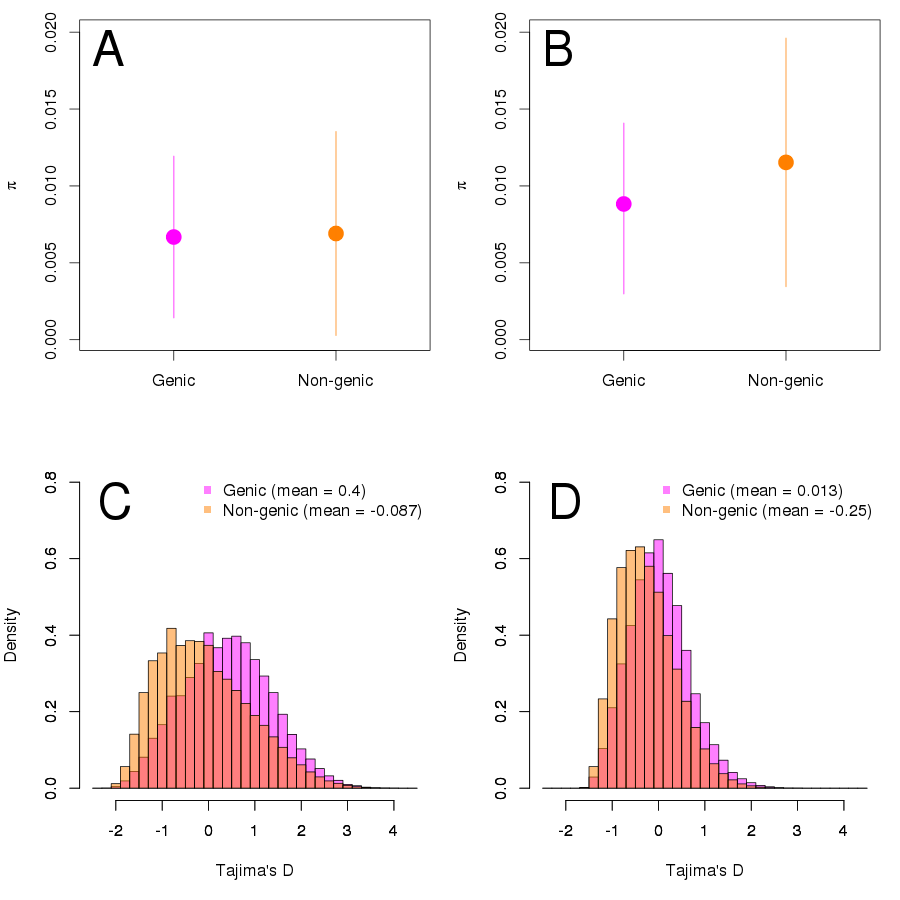
\includegraphics[width=.4\textwidth] {FigsAndFiles/Pi_and_Tajima.png}
\end{center}
\caption{Pairwise diversity $\pi$ (A,B) and Tajimas D (C,D) in 1kb windows from genic and nongenic regions of maize (A,C) and teosinte (B,D). Shown in A and B are means and one standard deviation.   \label{fig:diversity} }
\end{figure}

\subsection{Hard sweeps do not explain diversity differences}
Selection acting to increase the frequency of a new beneficial mutation will leave a signature of reduced diversity at surrounding linked sites \cite{smith1974}.
To evaluate whether patterns of such ``hard sweeps'' could explain observed differences in diversity between genic and non-genic regions of the genome, we compared diversity around missense and synonymous substitutions between \emph{Tripsacum} and either maize or teosinte (Figure
\ref{fig:hardSweeps}).
If a proportion of missense mutations have been fixed due to hard sweeps, diversity around these substitutions should be lower than around synonymous substitutions. 
We observe this pattern around the causative amino acid substitution in the the domestication locus \emph{tga1} (Figure \ref{sFig:tga1}), likely the result of a hard sweep during domestication \cite{wang2005origin, wang2015}.
Genome-wide, however, we observe no differences in diversity between synonymous and missense substitutions in either maize or teosinte.

\begin{figure*}
%\vspace*{.05in}
\centering
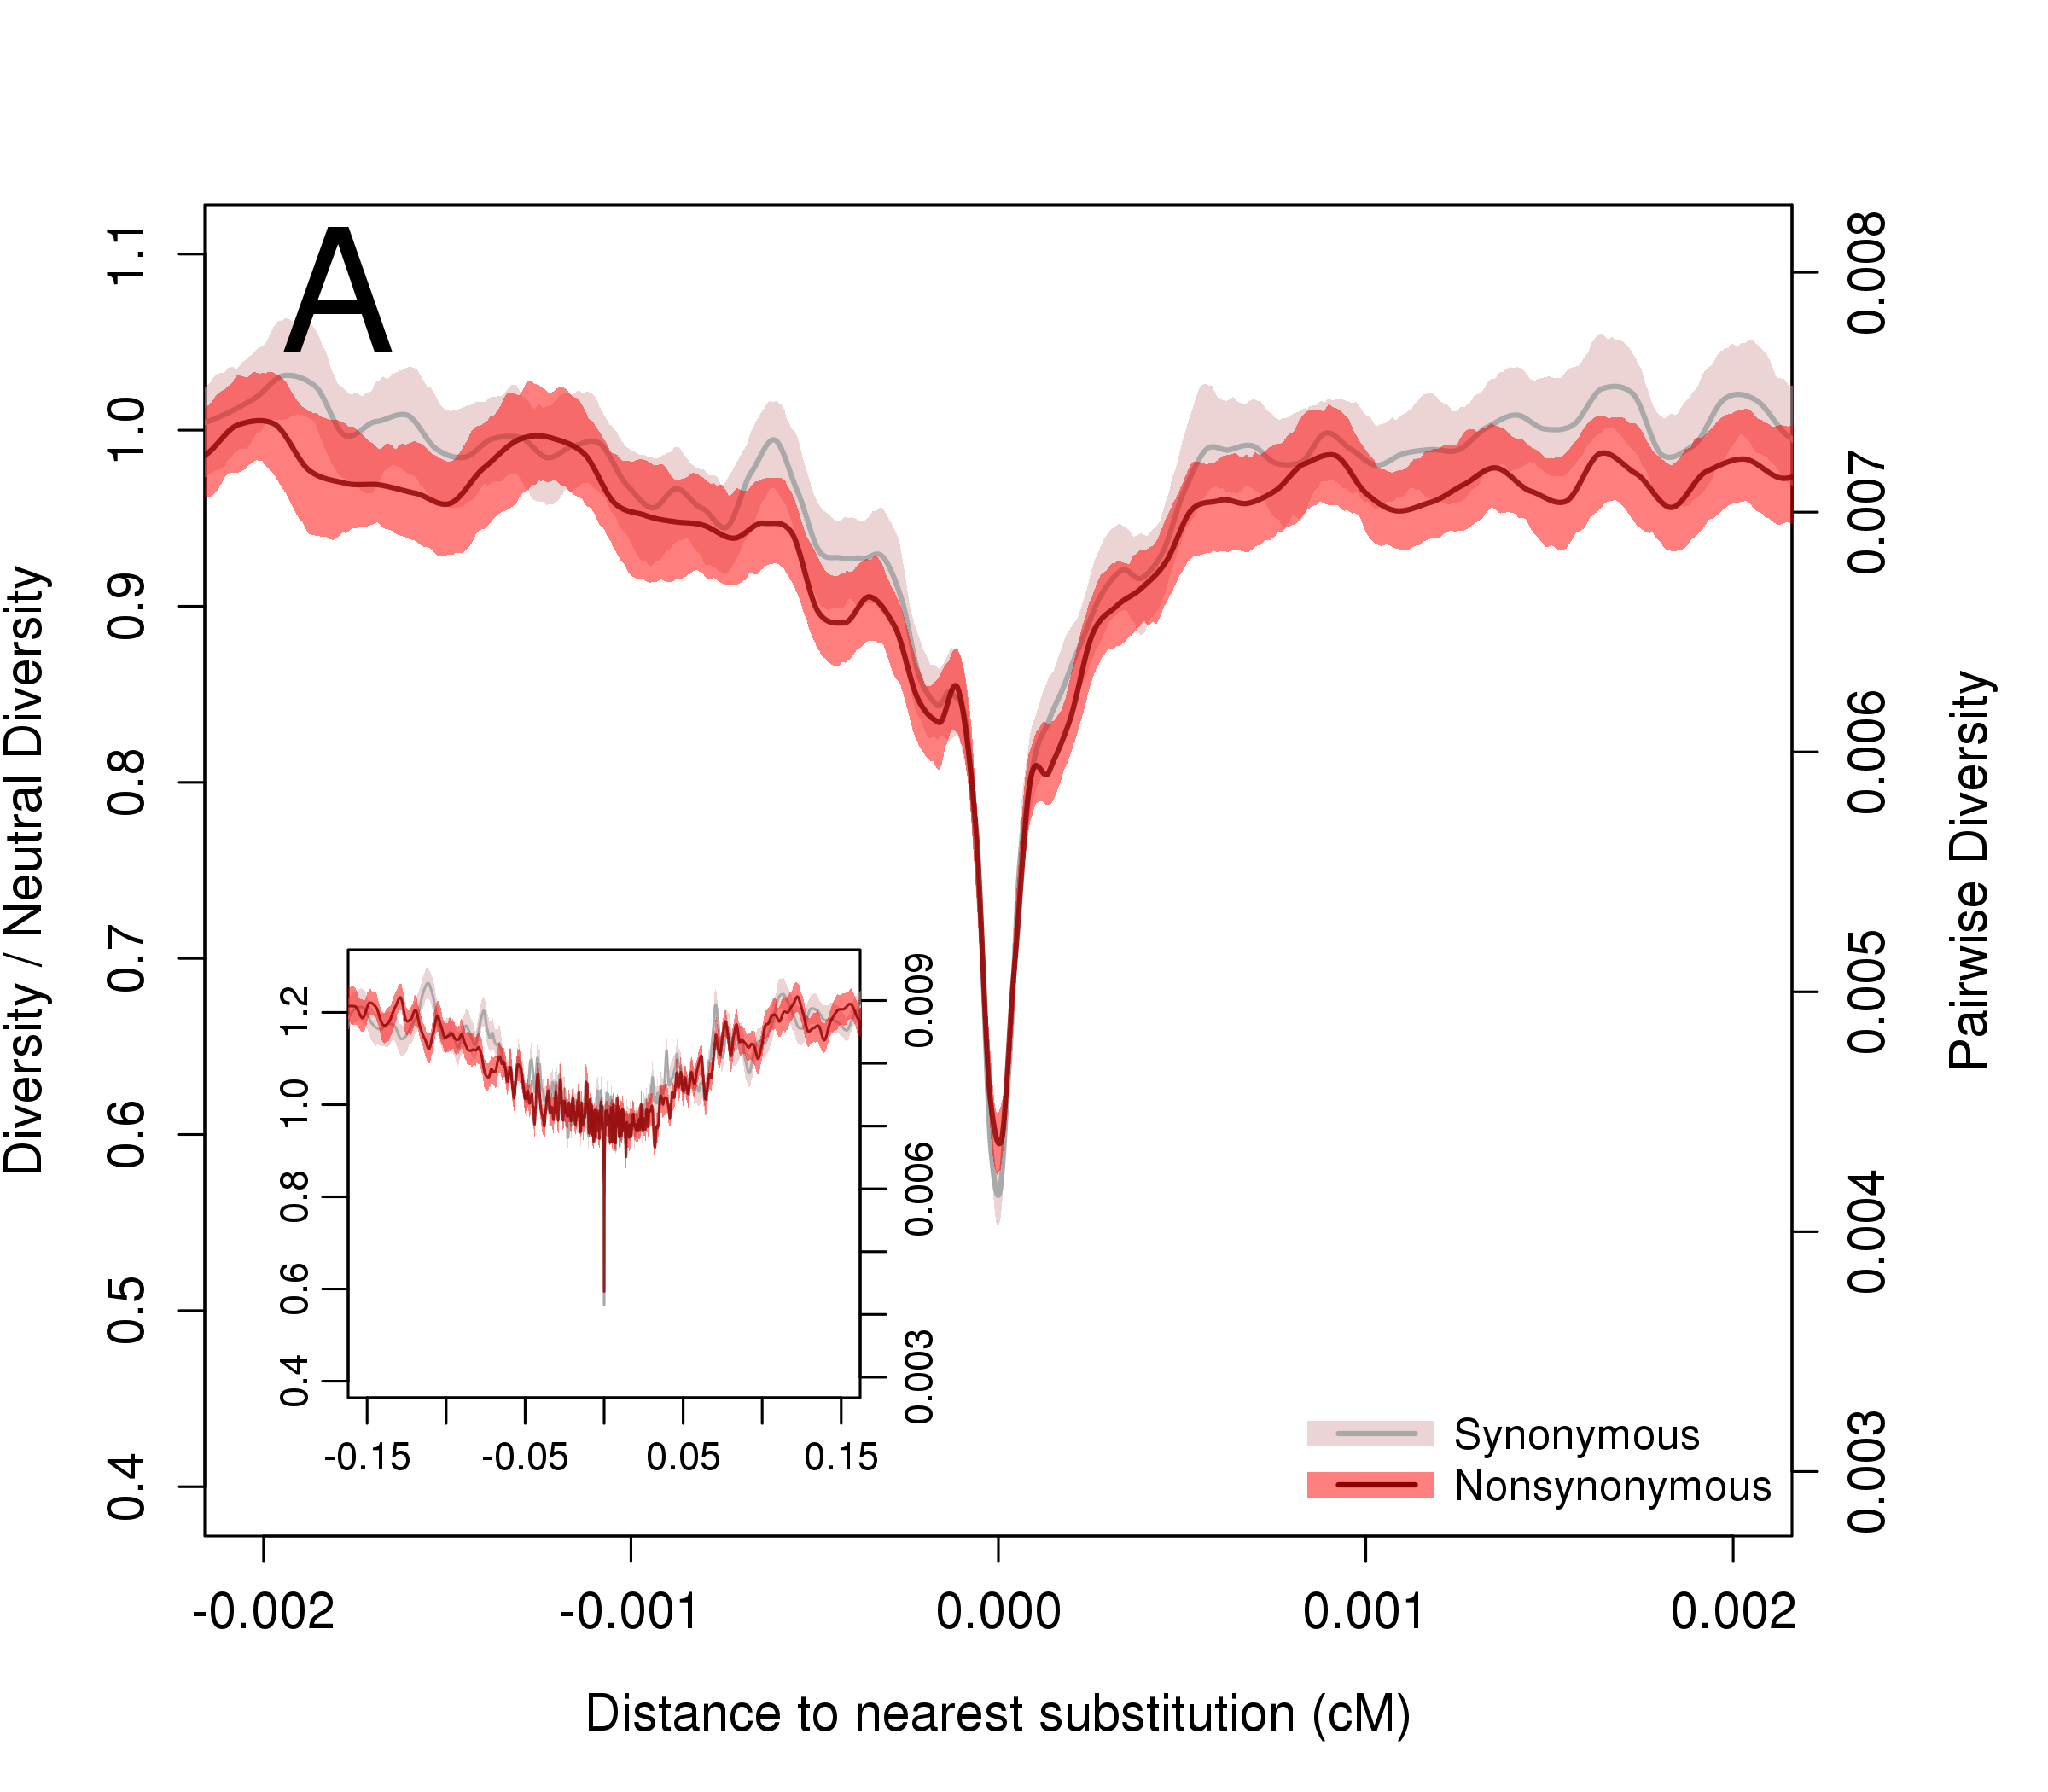
\includegraphics[width=.45\textwidth]{FigsAndFiles/plotDiversity_TvM_Folded2_Significance_Aug}
\hspace{0.05\textwidth} 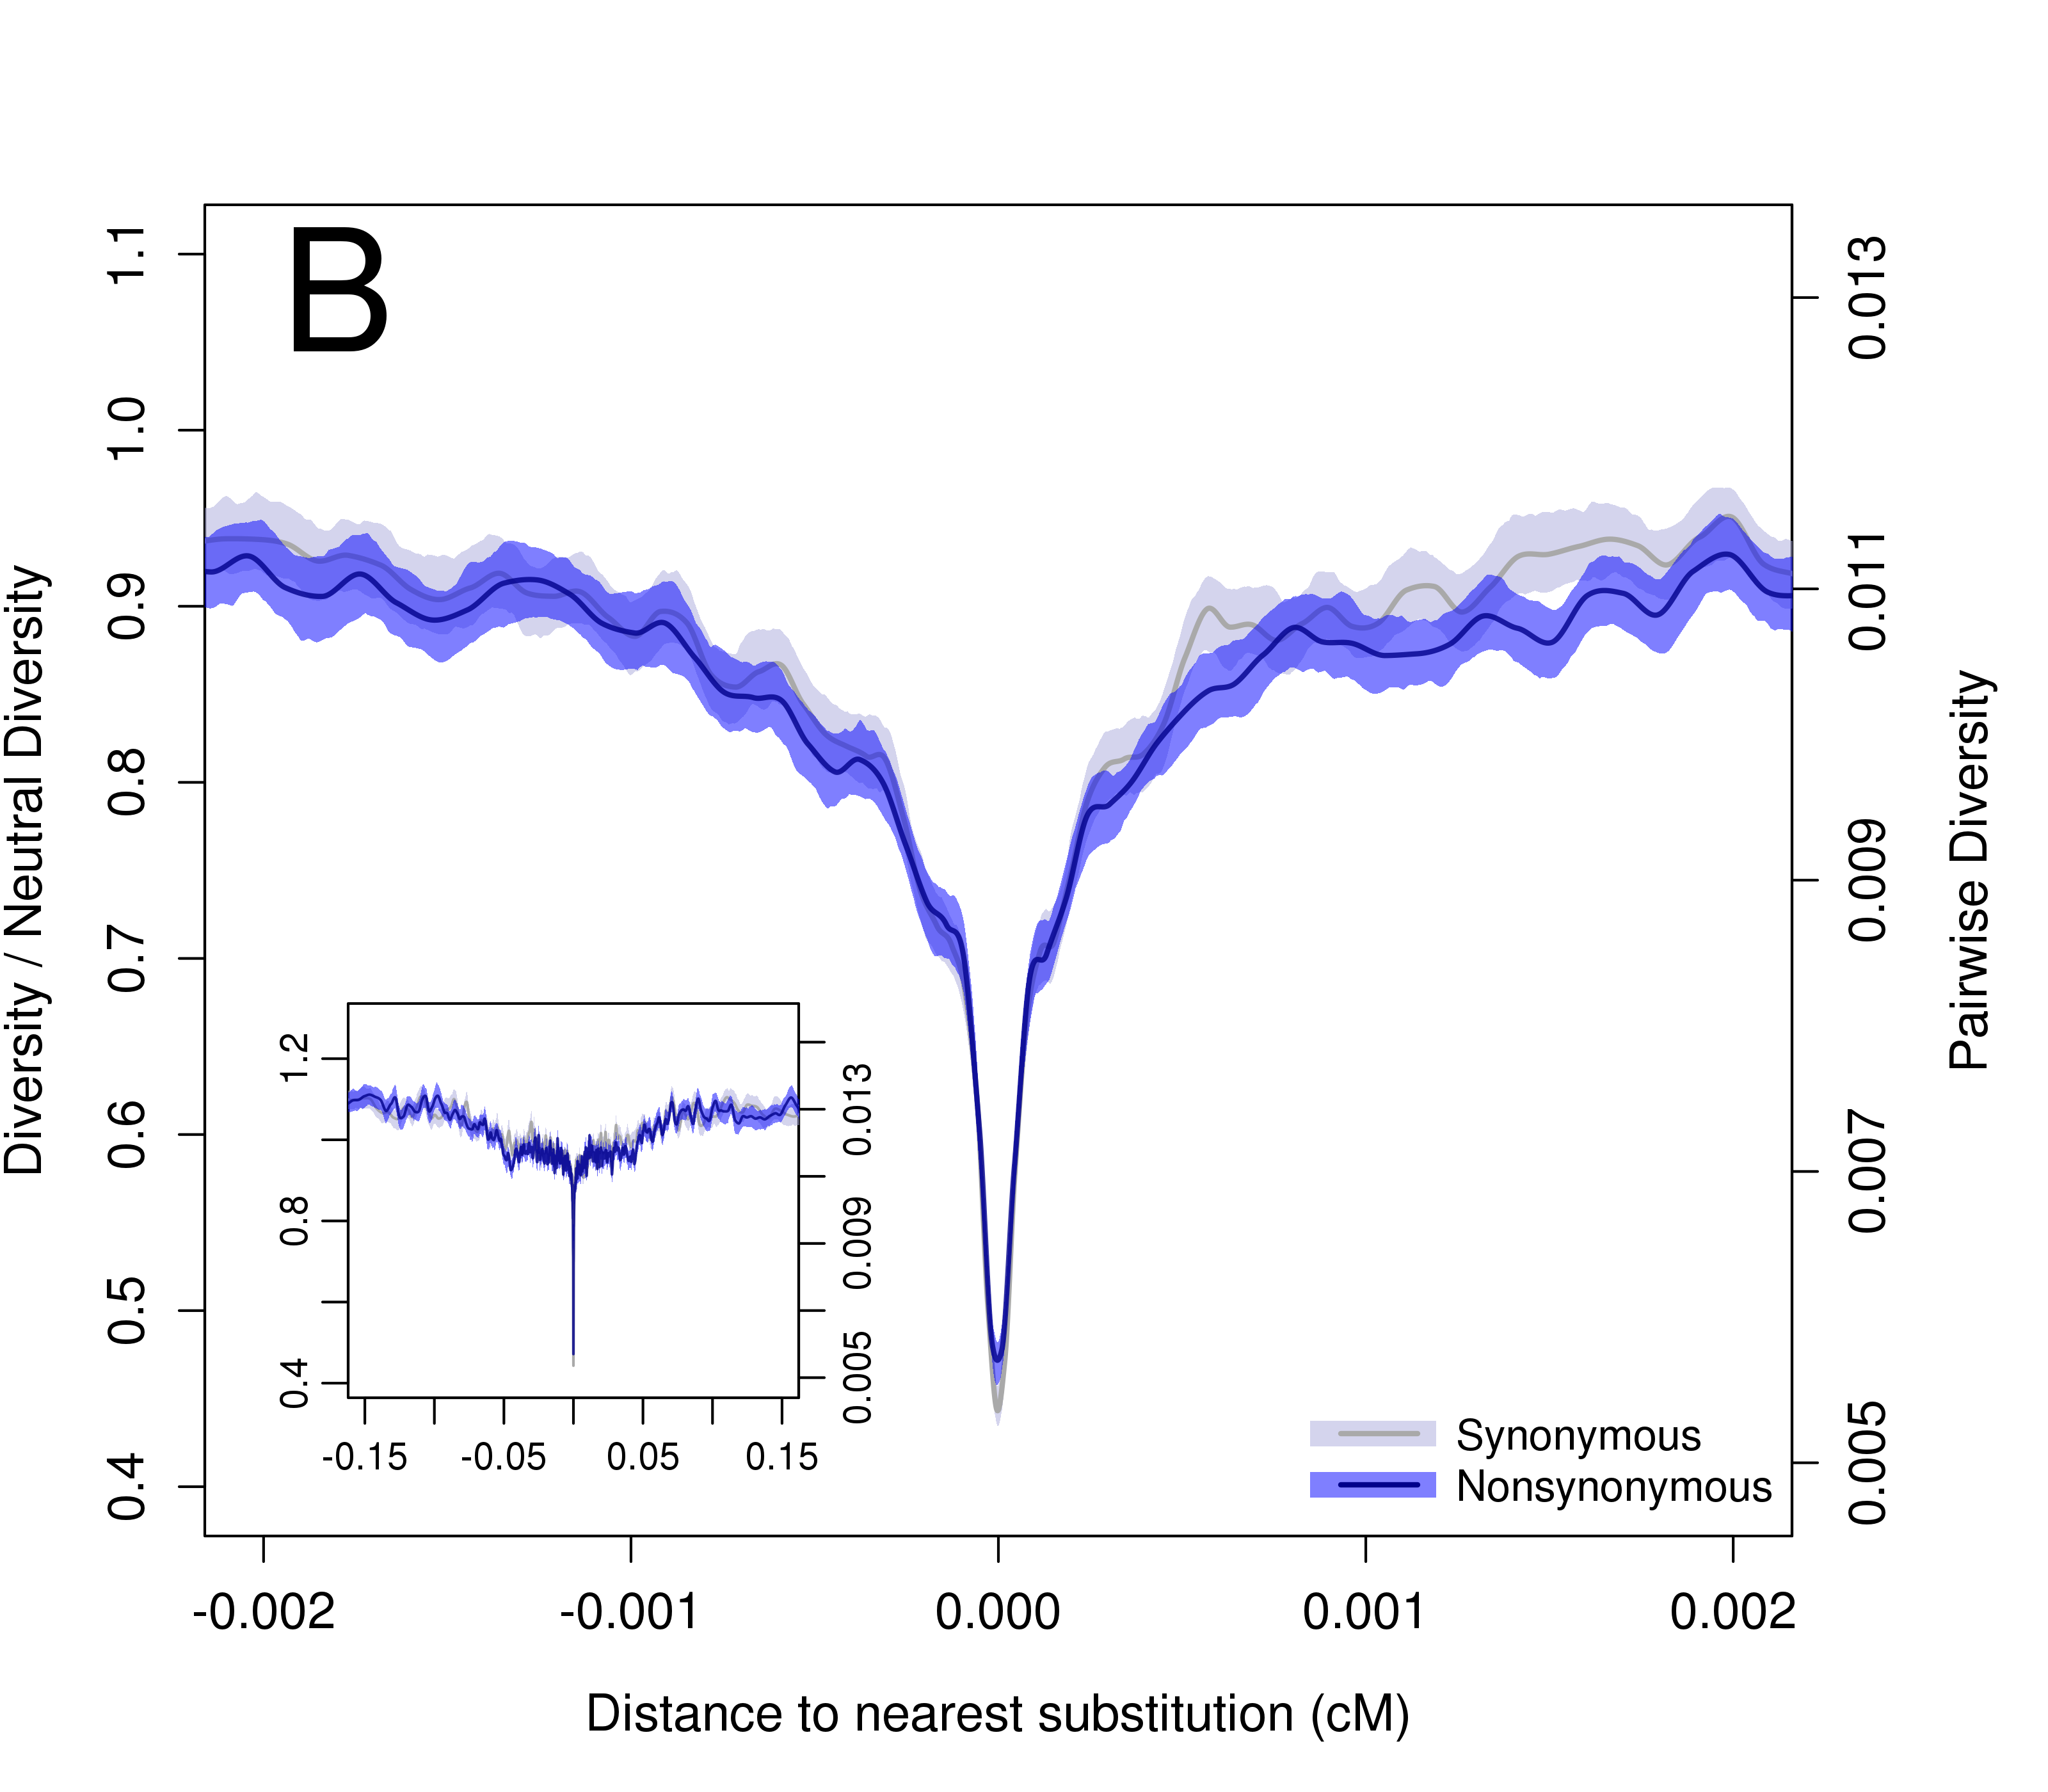
\includegraphics[width=.45\textwidth]{FigsAndFiles/plotDiversity_TvT_Folded2_Significance_Aug}
\caption{Pairwise diversity surrounding synonymous and non-synonymous (missense)
  substitutions in {\bf A} maize and {\bf B} teosinte. Axes show both absolute diversity values (on right) and values relative to mean nucleotide diversity in windows $\geq 0.01 cM$ from a substitution (on left).  Lines depict a loess curve (span of 0.01) and shading represents bootstrap-based 95\% confidence intervals. Inset plots depict a larger range on the x-axis. \label{fig:hardSweeps}}
\end{figure*}

Previous analyses have suggested that this approach may have limited power because a higher proportion of nonsynonymous substitutions will be found in genes under weak purifying selection and thus with higher genetic diversity \cite{enard2014}. 
To address this concern, we took advantage of genomic evolutionary rate profile (GERP) scores \cite{davydov2010}, a measure of evolutionary constraint, calculated across the maize genome \cite{rodgers2015}. 
We re-analyzed substitutions in subsets of genes with the highest and lowest 10\% quantile of mean GERP score, putatively representing genes under the strongest and weakest purifying selection  (Figure \ref{sFig:consUncons}). 
As expected, we see higher diversity around substitutions in genes under weak purifying selection, but we still see no difference between synonymous and missense substitutions in either subset of the data.
Taken together, these data suggest hard sweeps do not play a major role in patterning genic diversity in either maize or teosinte.

\subsection{Diversity is strongly influenced by purifying selection}

Selection can also reduce diversity in functional regions of the genome via removal of deleterious mutations, a process known to as purifying or background selection \cite{charlesworth1993}.
We investigated purifying selection in maize and teosinte by evaluating the reduction of diversity within genes.
Pairwise diversity is strongly reduced within genes for both maize and teosinte (Figure \ref{fig:purify}A) but recovers quickly at sites outside of genes, consistent with the low levels of linkage disequilibrium generally observed in maize \cite{tenaillon2002,chia2012}. 
The reduction in relative diversity is more pronounced in teosinte, however, reaching lower levels in genes and occurring over a wider region.  

Our initial comparison of synonymous and missense substitutions has low power to detect the effects of selection acting on multiple mutations or standing genetic variation, because in such cases diversity is not necessarily reduced \cite{innan2004,messer2013}. 
Such ``soft sweeps'', however, are still expected to occur more frequently in functional regions of the genome and could provide an alternative explanation for the observed reduction of diversity in genes. 
To test this possibility, we performed a genome-wide scan for selection using a method expected to be reasonably sensitive to both hard and soft sweeps \cite{garud2015}. 
After removing genes in the top 20\% of the H12 statistic used to identify targets of selection, we observe that qualitative differences between maize and teosinte in patterns of diversity in and near genes remained unchanged (Figure \ref{sFig:H12}A).

We interpret these combined results as suggesting that purifying selection has left a more pronounced signature in the teosinte genome due to the increased efficacy of selection resulting from differences in effective population size.\jri{weird that this is a 1-sentence paragraph?} 

\begin{figure*}
%\vspace*{.05in}
\centering
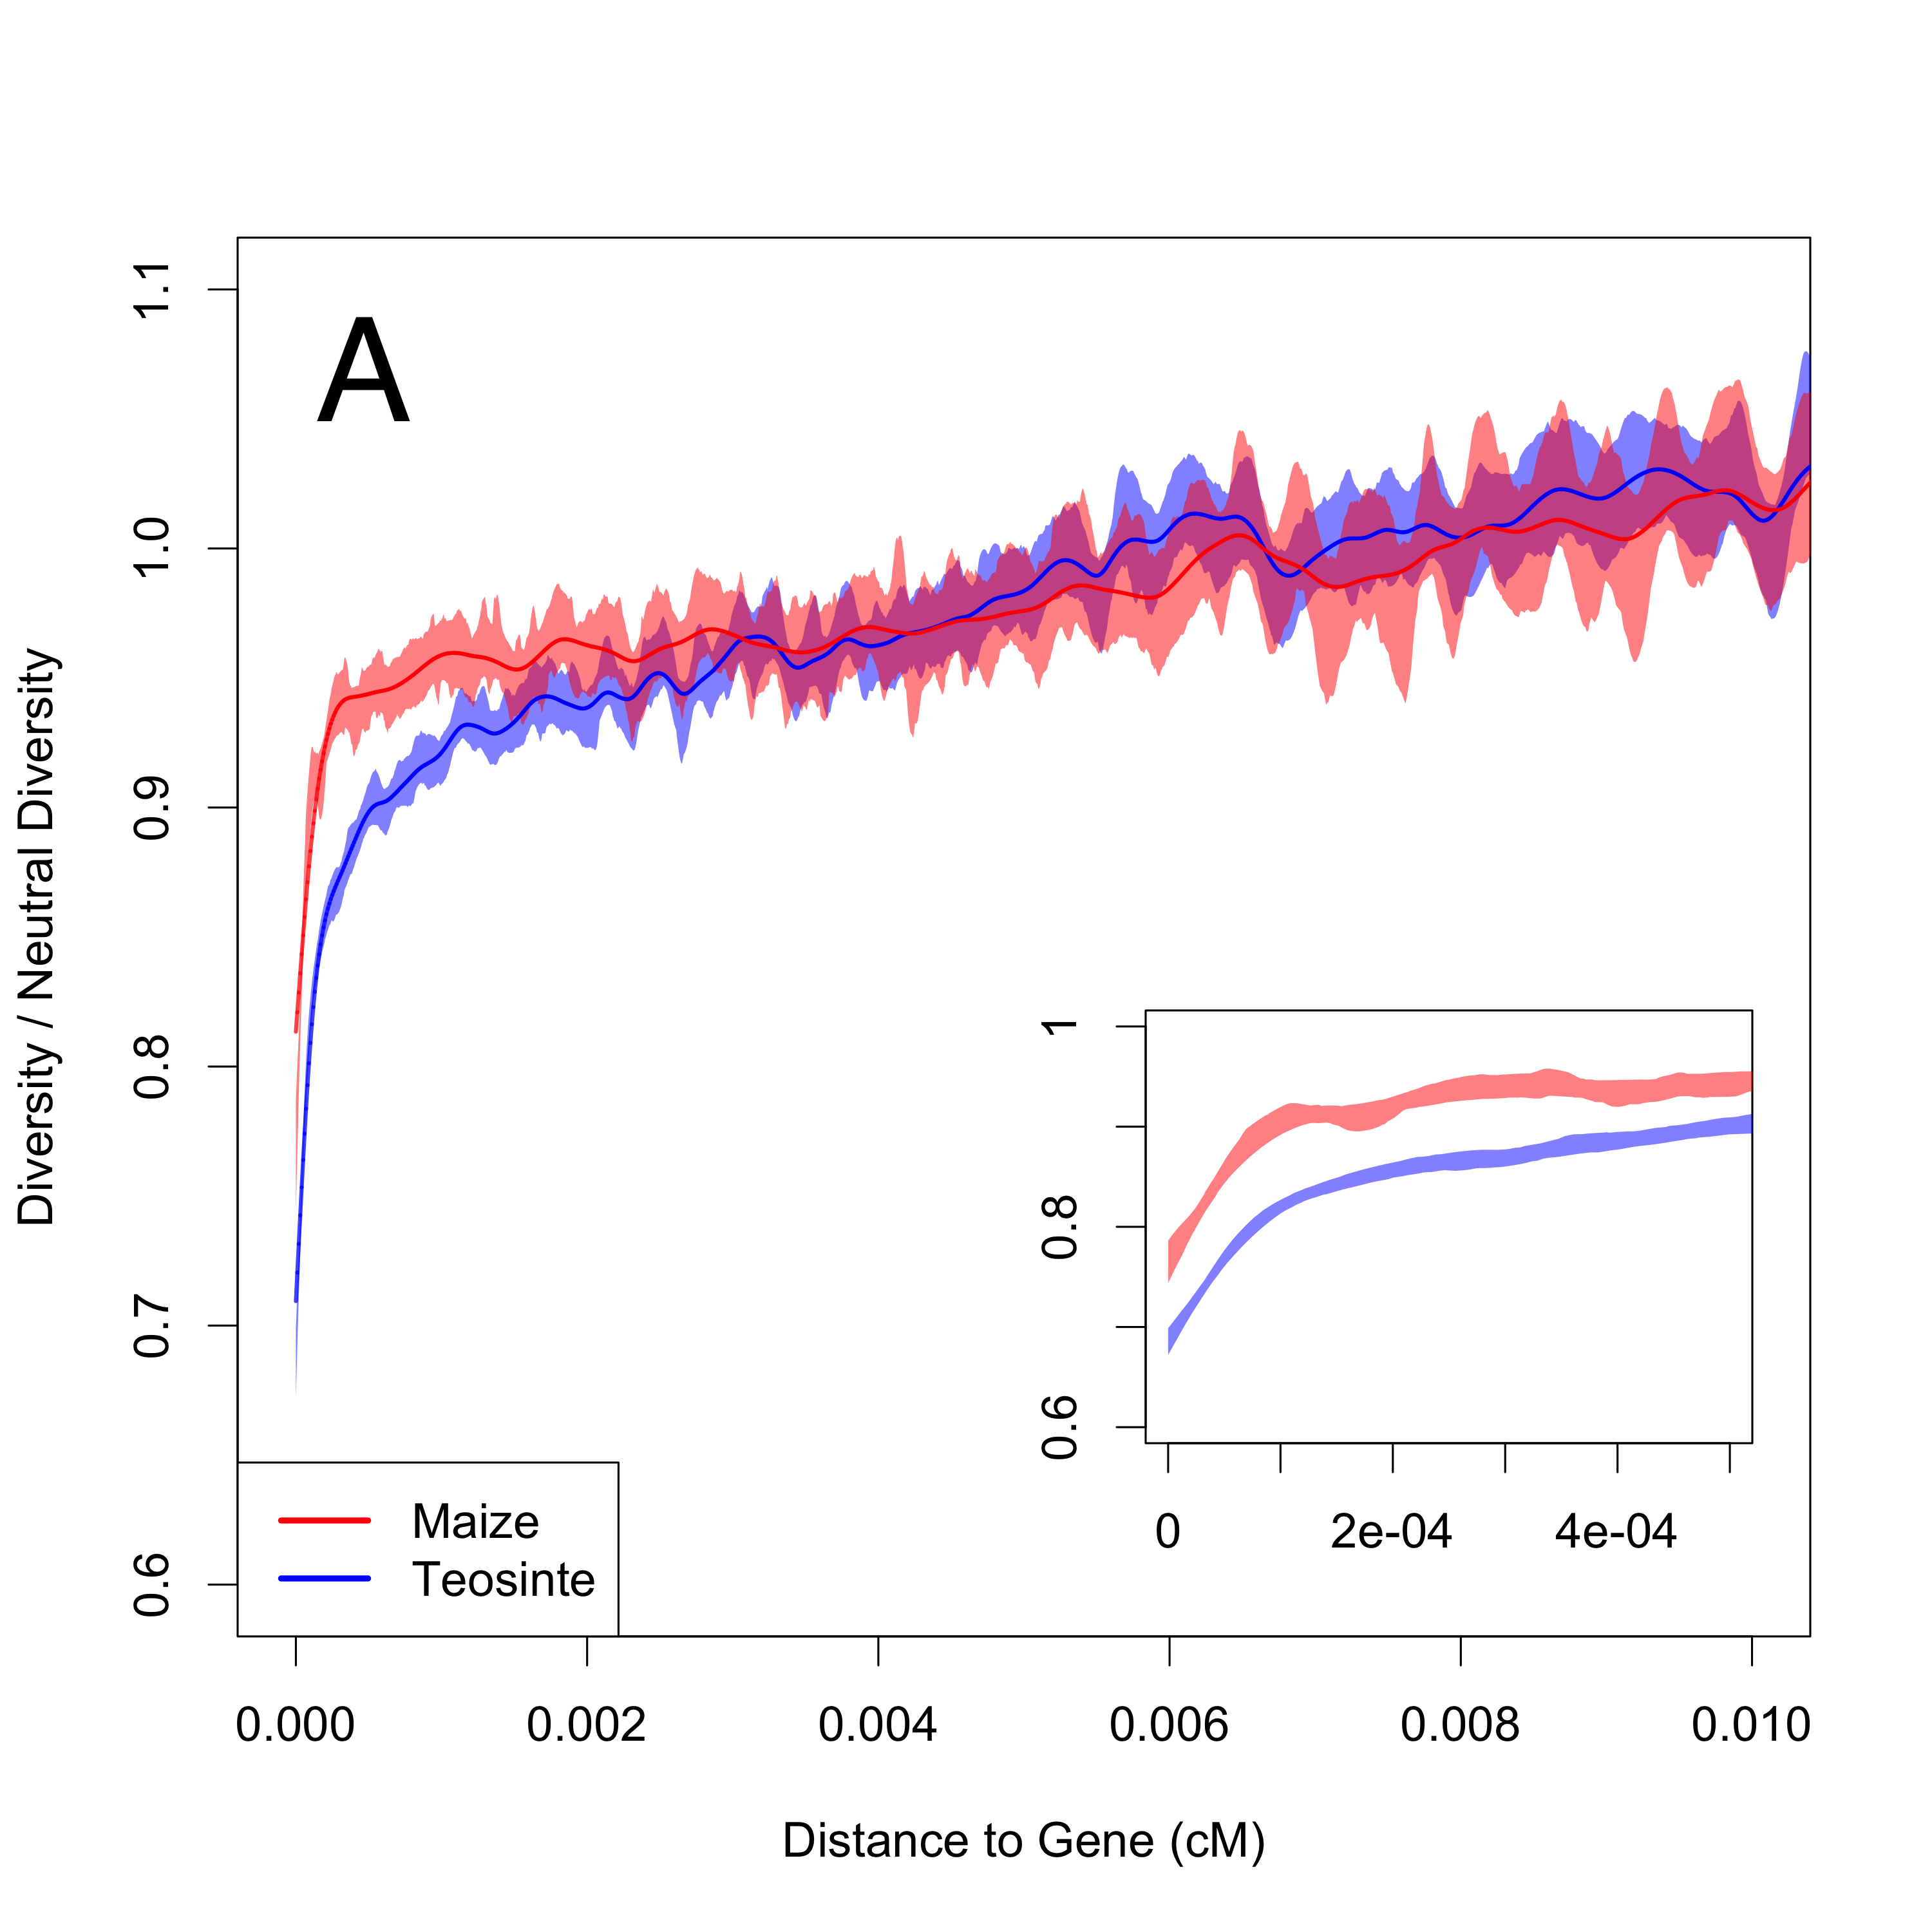
\includegraphics[width=.45\textwidth]{FigsAndFiles/distanceToGene_WithSignificance_Folded2_manuscript.png} 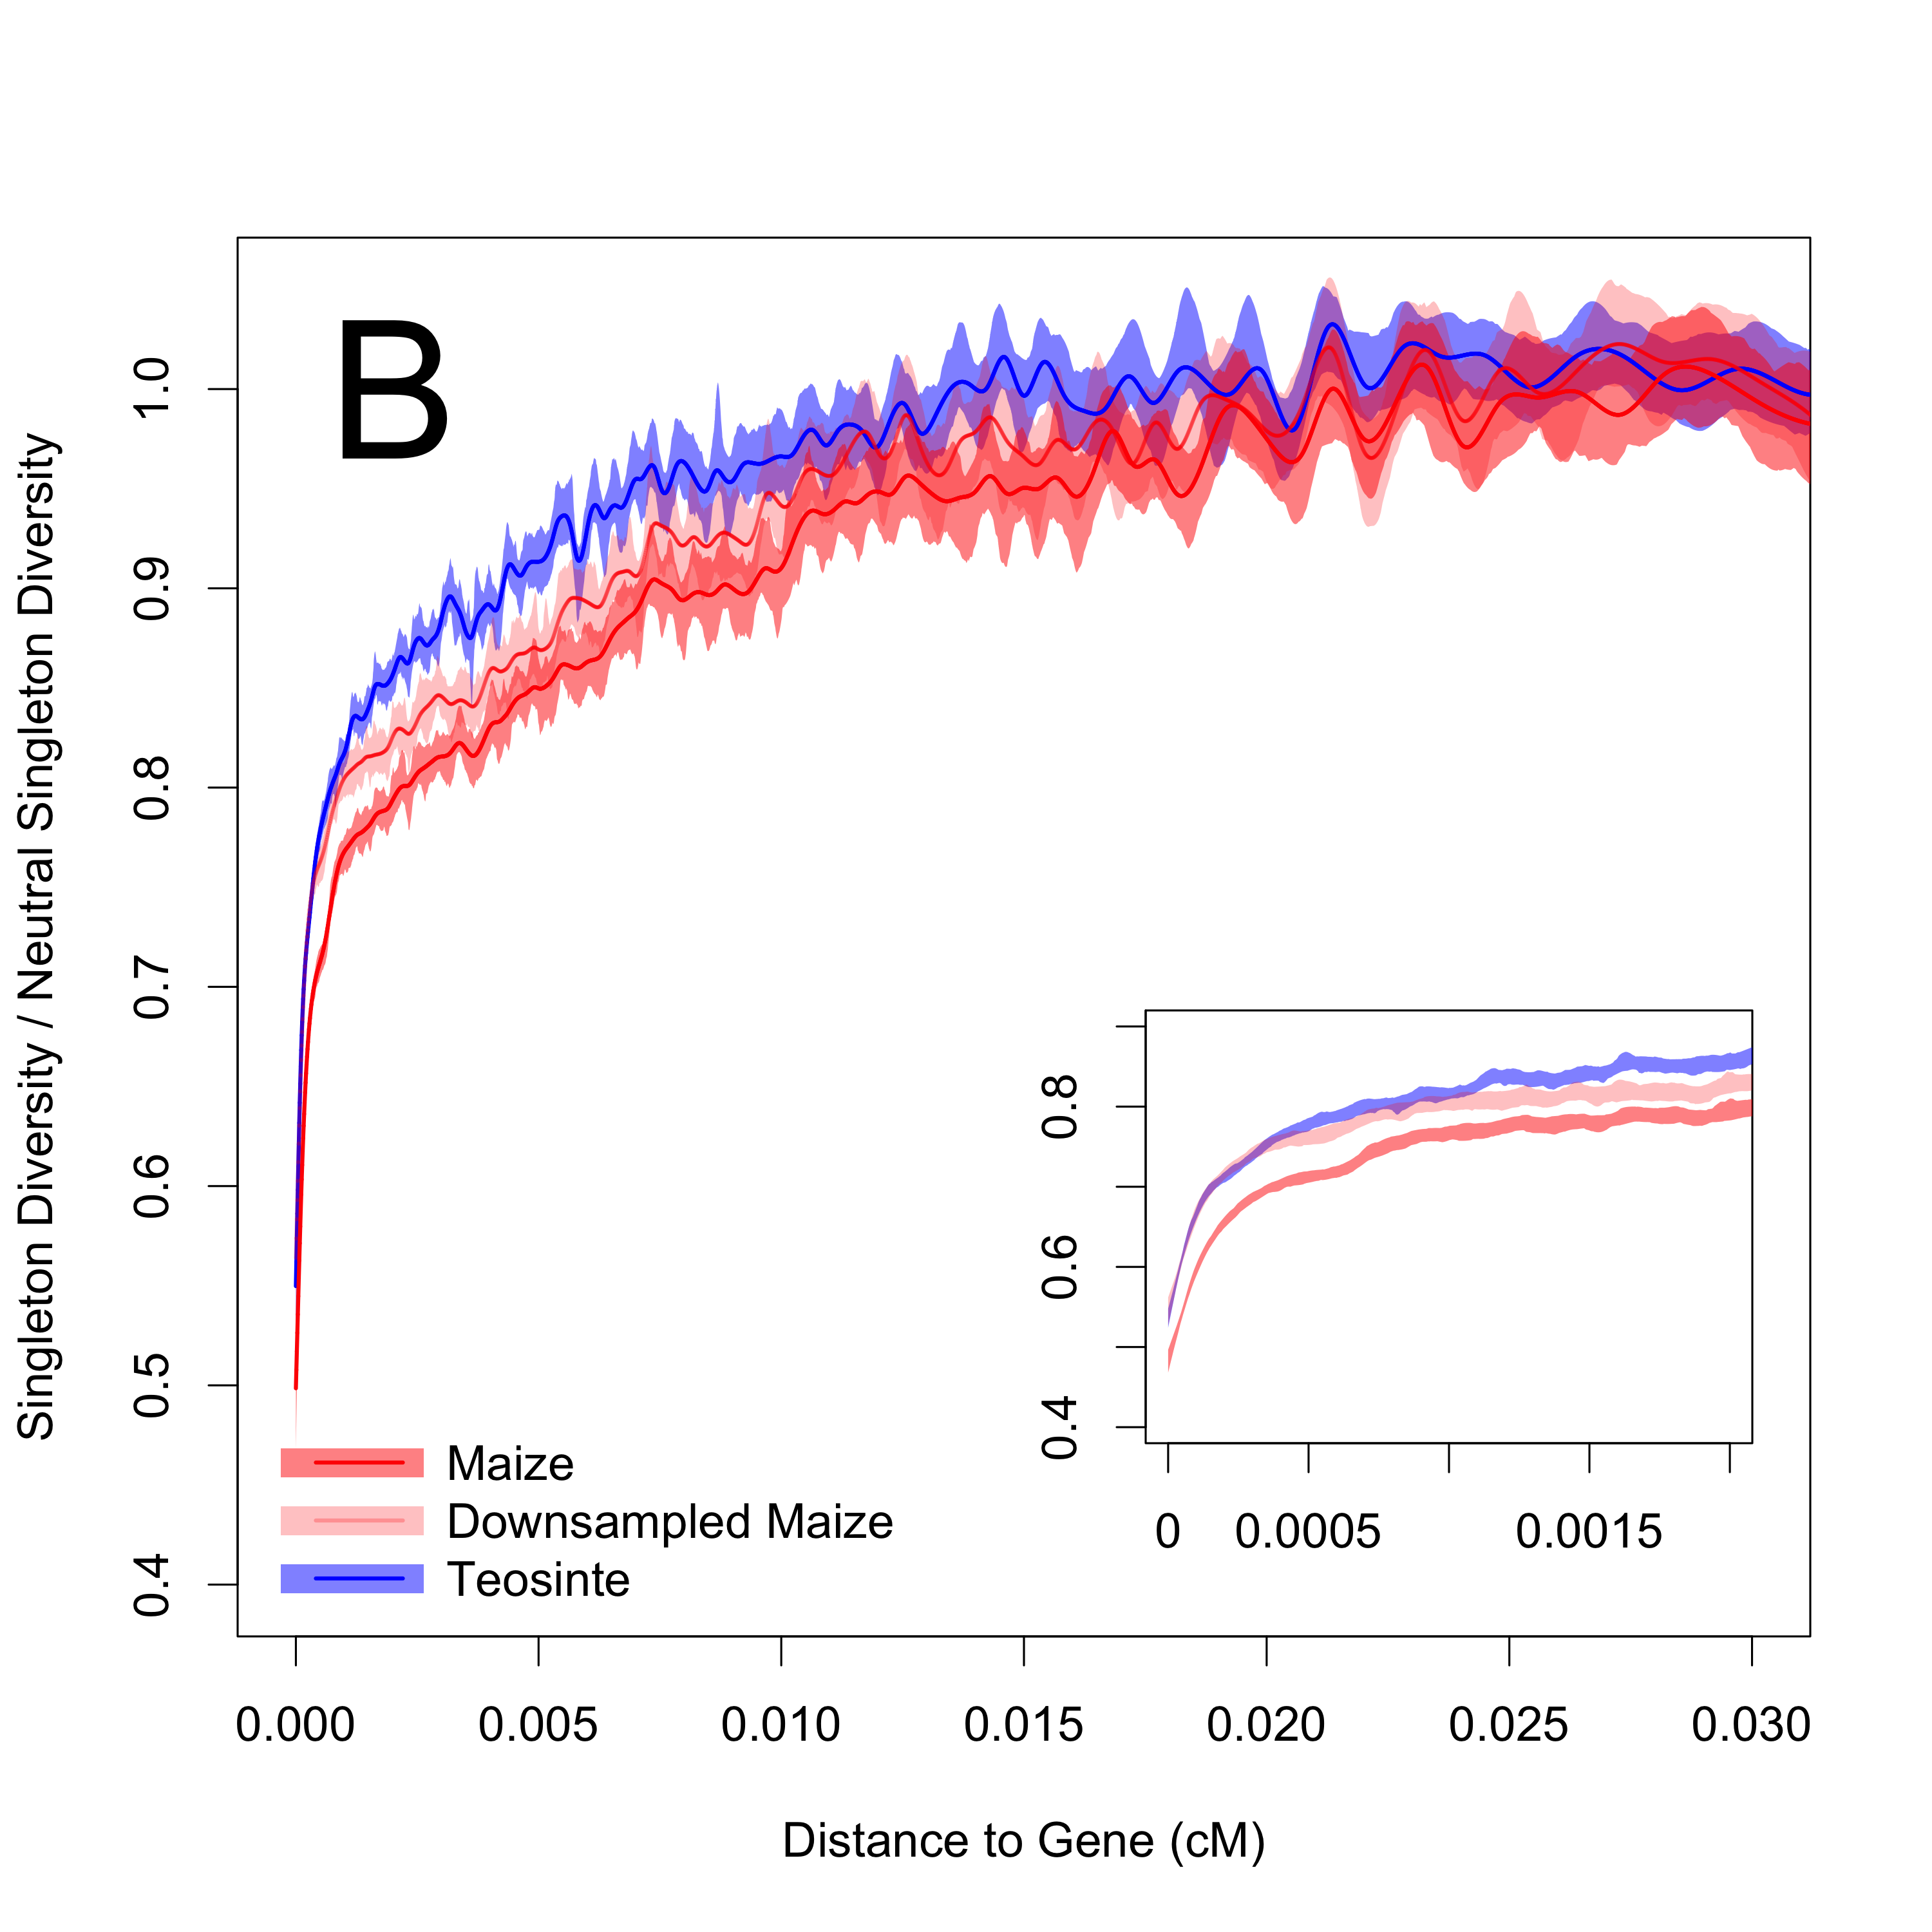
\includegraphics[width=.45\textwidth]{FigsAndFiles/distanceToGene_WithSignificance_Singletons_Downsampled_threeLines_manuscript.png}
\caption{Relative diversity versus distance to nearest gene in maize and teosinte. 
Shown are \textbf{A} pairwise nucleotide diversity and \textbf{B} singleton diversity.  
Relative diversity is calculated compared to the mean diversity in windows $\geq 0.01 cM$ or $\geq 0.02 cM$ from the nearest
gene for pairwise diversity and singletons, respectively. 
  Lines depict cubic smoothing splines with smoothing parameters chosen via generalized cross validation and shading depicts bootstrap-based 95\% confidence intervals.
  Inset plots depict a smaller range on the x-axis. \label{fig:purify}
  }
\end{figure*}

\subsection{Demography of maize domestication}
To explore whether differences in the efficacy of purifying selection between maize and teosinte can be explained by demographic processes, we estimated the parameters of a simple domestication bottleneck model  (Figure \ref{fig:bottleneck}). 
The most likely model estimates an ancestral population mutation rate of $\theta=0.0147$ per bp, which translates to an effective population size of $N_a \approx 123,000$ individuals given the mutation rate \cite{clark2005}.
The maize population splits from teosinte $\approx 15,000$ generations in the past with an initial size of only $\approx 5\% $ of ancestral $N_a$. 
Following domestication we estimate considerable gene flow between the populations: $M_{tm} =  1.1 \times 10^{-5} \times N_a $  migrants per generation from teosinte to maize and $M_{mt} =  1.4 \times 10^{-5} \times N_a$ migrants from maize to teosinte. 
After its split from teosinte our model posits exponential population growth in maize, estimating a final modern effective population size of $N_m \approx 370,000$.

\begin{figure*}
%\vspace*{.05in}
\centering
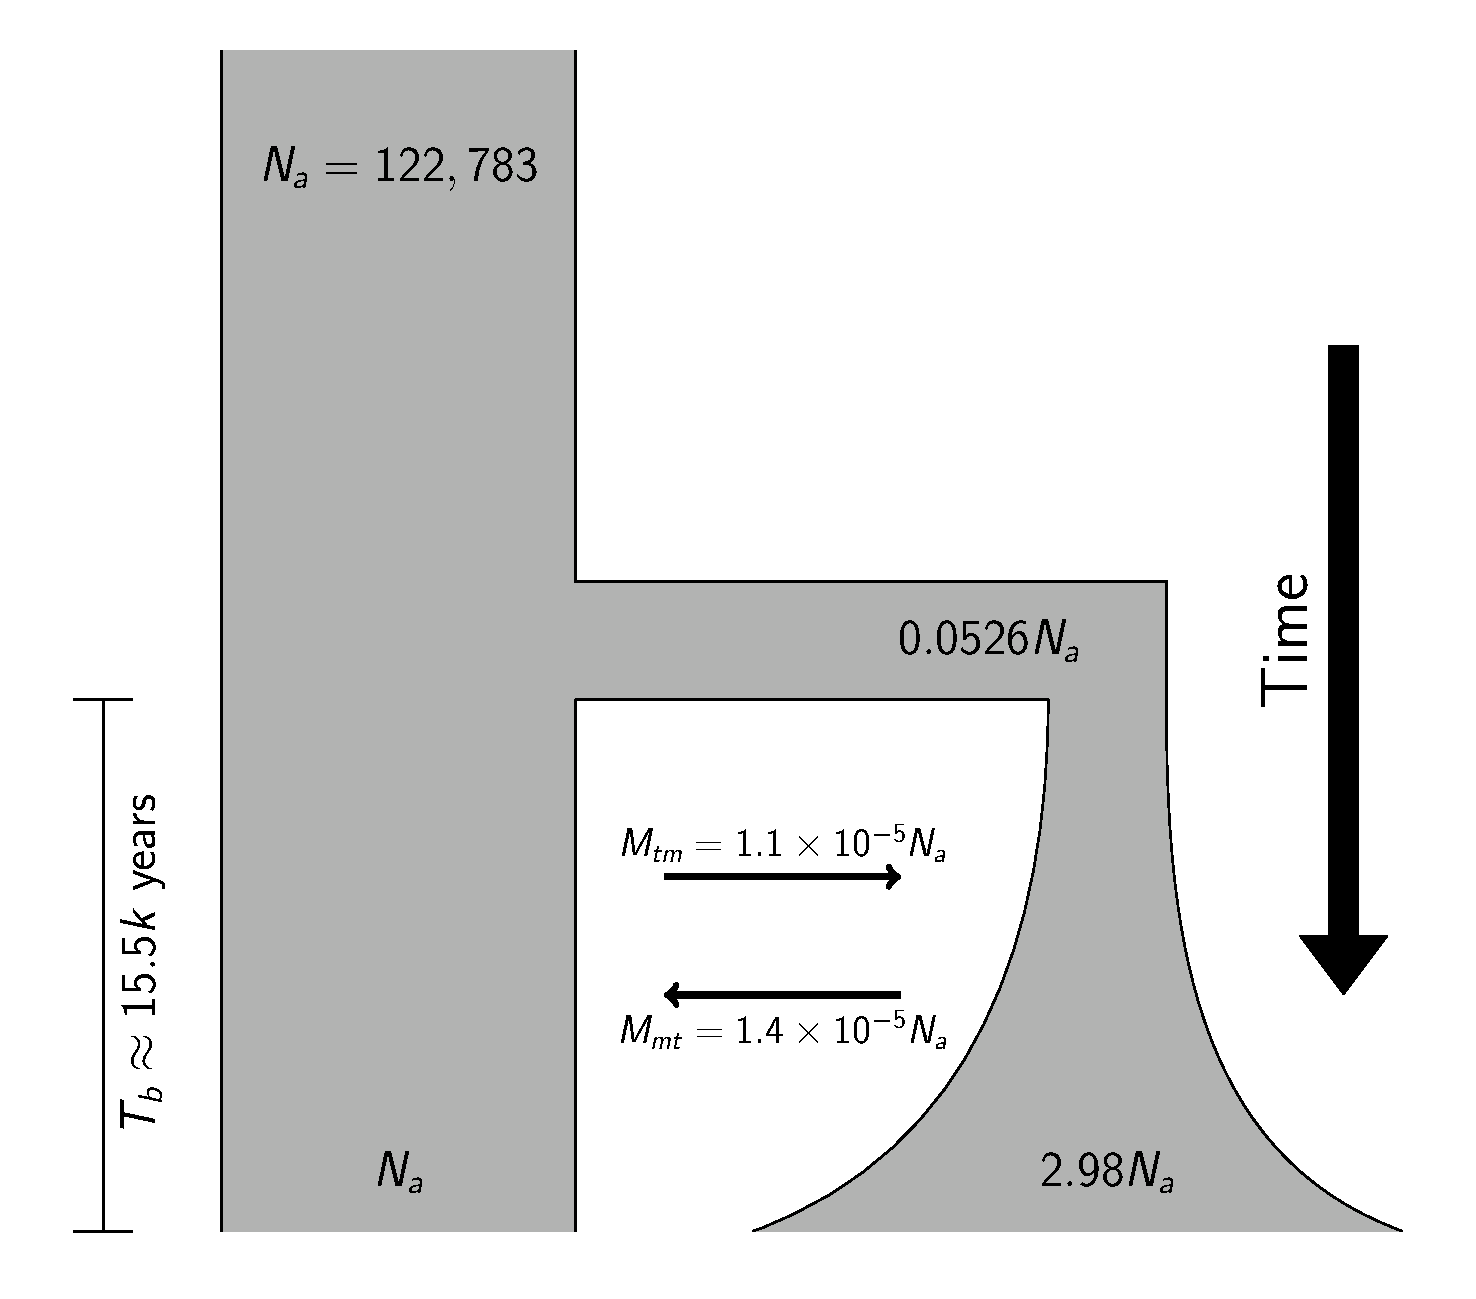
\includegraphics[width=.4\textwidth]{FigsAndFiles/DomesticationModel/domesticationModel.pdf}
\caption{Parameter estimates for a simple bottleneck model of maize domestication. See methods for details. \label{fig:bottleneck} }
\end{figure*}

Because our relatively small sample size limits our ability to characterize the rare variants that are most informative of population expansion, we took advantage of a complementary data set of more than 4,000 maize landraces collected from across the Americas \cite{Hearne2015} to estimate the modern maize effective population size from low frequency variants. 
This analysis yields a much higher estimate of the modern maize effective population size at  $N_m \approx 993,000$.

Finally, we reconstructed the demographic history of maize and teosinte using a recently developed coalescent approach \cite{schiffels2014}  that does not require conditioning on a particular model.
Though this analysis suggests the potential for nonequilibrium dynamics in teosinte, it nonetheless is broadly consistent with our simple model,   identifying a clear domestication bottleneck followed by rapid population expansion (Figure \ref{sFig:msmc}). 

\subsection{Population expansion leads to stronger purifying selection in modern maize}
Motivated by the rapid post-domestication expansion of maize evident from our demographic analysis, we investigated whether patterns of diversity at low frequency --- and therefore on average younger --- polymorphisms would show similar results in comparisons of maize and teosinte.
We thus repeated our analysis of diversity using alleles present in only a single individual in the sample.
In direct contrast to patterns observed for pairwise nucleotide diversity (Figure \ref{fig:purify}A), diversity of singletons was more strongly reduced in and near genes in maize than in teosinte (Figure \ref{fig:purify}B), even after downsampling our maize data to account for differences in sample size. This relationship was maintained when we analyzed diversity surrounding genes that did not show evidence of hard or soft sweeps according to H12 (Figure \ref{sFig:H12})
Finally, while direct comparison of curves for pairwise and singleton diversity within taxa are consistent with at least some non-equilibrium dynamics in teosinte, as indicated by our coalescent-based demographic analysis, these too reveal much stronger differences in maize (Figure \ref{sFig:singletonPi}). 

These results suggest that demographic history and population size change have impacted the efficacy of purifying selection during maize evolution.
In contrast, analysis of singleton diversity around missense and synonymous substitutions (Figure \ref{sFig:singleton}) provides a nearly identical pattern to that shown in Figure \ref{fig:hardSweeps}, providing little support for a substantial increase in the number or strength of hard sweeps occurring in maize.  

\section{Discussion}

\subsection{Hard sweeps do not shape genome-wide diversity in maize}

Our findings demonstrate that classic hard selective sweeps have not contributed substantially to genome-wide patterns of diversity in maize, a result we show is robust to concerns about power due to the effects of background selection  \cite{enard2014}. 
Although our approach ignores the potential for hard sweeps in noncoding regions of the genome, a growing body of evidence argues against hard sweeps as the prevalent mode of selection shaping maize variability. 
Among well-characterized domestication loci, only the gene \emph{tga1} shows evidence of a hard sweep on a missense mutation \cite{wang2015}, while several loci are consistent with ``soft sweeps''  from standing variation \cite{studer2011,gallavotti2004role} or multiple mutations \cite{wills2013}. 
Moreover, genome-wide studies of domestication \cite{hufford2012},  local adaptation \cite{Takuno15062015} and modern breeding \cite{beissinger2014} all support the importance of standing variation as the primary source of adaptive variation. 
Soft sweeps are expected to be common when $2N_e\mu_b \ge 1$, where $\mu_b$ is the mutation rate of beneficial alleles with selection coefficient $s_b$ \cite{messer2013population}.  
Assuming a mutation rate of $3 \times 10^{-8}$ \citep{clark2005} and that on the order of $\approx 1-5\%$ of mutations are beneficial \citep{eyre2007distribution}, this implies that soft sweeps should be common in both maize and teosinte for mutational targets $>>10kb$ --- a plausible size for quantitative traits or for regulatory evolution targeting genes with large up- or down-stream control regions \citep[e.g.][]{studer2011}. \jri{no mention of our H12 results. I think that's OK?}

\jri{paragraph needs work. maybe eliminate/move? i do think we need some comparison to other stuff, but the broader Ne-selection efficiency argument should come later.}
The absence of evidence for a genome-wide impact of hard sweeps differs markedly from observations in \emph{Drosophila} \cite{sattath2011} and \emph{Capsella} \cite{williamson2014}, but is consistent with data from humans \cite{hernandez2011,pritchard2010genetics}. 
In a related study, \cite{corbett2015} showed that selection tends to have an elevated impact on reducing diversity in species with large population size compared to small. This may explain why maize and humans, both bottlenecked species, show similar patterns while drosophila and capsella behave differently. \textcolor{red}{However, we also do not observe abundant hard sweeps in teosinte, which calls this explanation into question.}

\subsection{Demography of domestication}
Although a number of authors have investigated the demography of maize domestication \cite{eyre1998, tenaillon2004selection, wright2005}, these  efforts relied on data only from genic regions of the genome and made a number of limiting assumptions about the demographic model.  
We show that diversity within genes has been strongly reduced by the effects of linked selection, such that even synonymous polymorphisms in genes are not representative of diversity at unconstrained sites.  
By utilizing the full joint SFS, we are able to estimate population growth, gene flow, and the strength of the domestication bottleneck without requiring assumptions about its duration.  

One surprising result from our model is the estimation of the timing of domestication at $\approx 15,000$ years before present.
While this appears to conflict with archaeological \cite{piperno2009starch} estimates, we instead argue this estimate reflects the fact that the genetic split between populations likely preceded anatomical changes that can be identified in the archaeological record. 
We also note that our result may also be inflated due to population structure, as our geographically diverse sample of teosinte may include populations diverged from those that gave rise to maize.

The estimated bottleneck of $\approx 5\%$ of the ancestral teosinte population seems low given that maize landraces exhibit $\approx 80\%$ of the diversity of teosinte \citep{hufford2012}, but our model suggests that the effects of the bottleneck on diversity are likely ameliorated to some extent by both gene flow and rapid post-domestication growth (Figure \ref{fig:bottleneck}).   
Although we estimate that the modern effective size of maize is larger than teosinte, the small size of our sample reduces our power to identify the low frequency alleles most sensitive to rapid population growth \cite{keinan2012}.  
A better estimate comes from our analysis of singleton diversity in a large sample of maize landraces \cite{Hearne2015}, which suggests a modern effective size of $\approx 1$ million, or nearly eight times higher than modern teosinte.
Even this estimate, however, is likely downwardly biased due to missing data, sample size, and ascertainment in the genotyping data.
An alternative approach is to use estimates of the census size of modern maize: there are 47.9 million ha of open-pollinated maize in production \cite{cimmyt1999}, likely planted at a density of $\approx 25,000$ individuals  per hectare \cite{baden2001culture}.
Assuming the effective size is only $\approx 0.4\%$ of the census size (i.e. 1 ear for every 1000 plants), this still implies a modern effective population size of more than four billion.
While these rough estimates are likely poor, all of the evidence points to the fact that the effective size of modern maize is extremely large.

\subsection{Demography influences the efficiency of purifying selection}
\jri{section needs help --  i'm not happy with the writing} 
We find a more pronounced decrease in nucleotide diversity around genes in teosinte compared to domesticated maize (Figure \ref{fig:purify}A).
This difference in diversity is likely due to the effects of purifying selection.
Purifying selection is more efficient in larger populations  \cite{kimura1984}, and our observation is thus consistent with our demographic model and previous work \cite{eyre1998, tenaillon2004selection, wright2005, ross2009} showing a smaller long-term effective population size in maize.  
To understand how recent population growth has changed the effects of linked selection, we also analyzed diversity of singleton polymorphisms.   Under a simple neutral model, lower frequency polymorphisms are expected to be younger, and patterns of diversity at singleton SNPs should thus represent recent evolutionary history. 
Consistent with its larger current size and thus more efficient purifying selection, we see a stronger decline of singleton diversity around genes in maize (Figure \ref{fig:purify}B than teosinte.

\jri{I would like to see a supplemental figure or maybe just number here on the partial correlation in both teosinte and maize of diversity with recombination after accounting for gene density.  do this in 500kb windows and then in 10kb windows.  we should do the correlation with both pi and singletons.  This let's us compare more explictly with studies like C-D who evaluate overall patterns of linked selection. will be especially cool if we don't see a big difference in big windows but we do in 10kb windows.  }
A consequence of the inefficient purifying selection that maize experienced during its bottleneck is likely that it harbors more weakly deleterious alleles segregating at intermediate frequency than does teosinte. This could be a part of the explanation of why maize inbreds have continued to improve over the past several decades \cite{meghji1984}; if deleterious alleles tend to be recessive and are particularly frequent, they will have ample opportunities to display their phenotypes in inbreds. Our results also demonstrate that recent purifying selection in maize has become much more effective, potentially explaining the ongoing improvement of these inbreds as maize lines are continuously selected. Additionally, the large $N_e$ of modern maize compared to modern teosinte implies that for new mutations, selection will operate much more efficiently in maize. \jri{inbreds stuff OK, but should be shortened.  and we need more/broader. Chia, Rogers-Melnick, Mezmouk all looked at load. does this have implications for large effect load (i.e. should bneck have purged those?), for heterosis, architecture of quant. traits, etc.}

\jri{these results have implications for lots of studies. recent demographic history often ignored (examples). in crops, bneck is considered and loss of diversity, but expansion also likely ubiquitous and consequences not well studied.  in humans XYZ, and we see some of that already here. this argues that a full understanding of diversity in both wild and cultivated plants will require recent demography. mention C-D ignored recent demography -- here's where rec/pi windows could help.}

\begin{materials}

\subsection{BASH, R, and Python scripts}
All scripts used for analysis are available in an online repository at \textcolor{red}{REPO ADDRESS HERE.} 

\subsection{Plant materials}
We made use of published sequences from inbred accessions of teosinte (Z. \emph{mays} ssp. \emph{parviglumis}) and maize landraces from the Maize HapMap3 panel as part of the Panzea project (bam files are available at \textcolor{red}{/iplant/home/shared/panzea/hapmap3/bam\_internal/v3\_bams\_bwamem}) \cite{chia2012, lemmon2014,hapmap3}. 
From these data, we removed 4 teosinte individuals that were not ssp. \emph{parviglumis} or appeared as outliers in an initial principal component analysis conducted with the package adegenet \cite{jombart2011} (Figure \ref{sFig:PCA}), leaving 13 teosinte and 23 maize that were used for all subsequent analyses (Table \ref{sTab:list}). We also utilized a single tripsacum (\emph{T. dactyloides}) individual as an outgroup (bam file available at \textcolor{red}{/iplant/home/shared/panzea/hapmap3/bam\_internal/v3\_bams\_bwamem}). \jri{some clarification here. did we use Lemmon's higher depth teosinte? If so, why does Li say we only had 7 high-depth bam files? there should be more}

\subsection{Physical and genetic maps}
Sequences were mapped to the maize B73 version 3 reference genome \cite{schnable2009} (ftp://ftp.ensemblgenomes.org/pub/plants/release-22/fasta/zea\_mays/dna/) as described by \cite{hapmap3}. All analyses made use of uniquely mapping reads with mapping quality score $\geq  30$ and bases with base quality score $\geq 20$; quality scores around indels were adjusted following Li \emph{et al.} \cite{li2011statistical}.
We converted physical coordinates to genetic coordinates via linear interpolation of the previously published 1cM resolution NAM genetic map \cite{glaubitz2014}. 

\subsection{Estimating the site frequency spectrum}
We estimated both the genome-wide site frequency spectrum (SFS) as well as a separate SFS for genic (within annotated transcript) and intergenic ($\geq 5kb$ from a transcript) regions. 
We used the biomaRt package \cite{durinck2009,durinck2005} of R \cite{R2014} to parse annotations from genebuild version 5b of AGPv3. 
We estimated single population and joint SFS with the software ANGSD \cite{korneliussen2014}, including all positions with at least one aligned read in $\geq 80\%$ of samples in one or both populations.
We assumed individuals were fully inbred and treated each line as a single haplotype. Because ANGSD cannot calculate a folded joint SFS, we first polarized SNPs using the maize reference genome and then folded spectra using $\delta\alpha\delta{i}$ \cite{gutenkunst2009}.

\subsection{Demographic inference}
We used the software $\delta\alpha\delta{i}$ \cite{gutenkunst2009} to estimate parameters of a domestication bottleneck from the joint maize-teosinte SFS, using only sites $>5 kb$ from a gene to ameliorate the effects of linked selection.
We modeled a teosinte population of constant effective size $N_a$, that at time $T_b$ generations in the past gave rise to a maize population of size $N_b$ which grew exponentially to size $N_m$ in the present (Figure \ref{fig:bottleneck}).
The model includes migration of $M_{mt}$ individuals each generation from maize to teosinte and $M_{tm}$ individuals from teosinte to maize.  We estimated $N_a$ using $\delta\alpha\delta{i}$'s estimation of $\theta=4N_a\mu$ from the data and a mutation rate of $\mu = 3 \times 10^{-8}$ \cite{clark2005}. 
We estimated all other parameters using 1,000 $\delta\alpha\delta{i}$ optimizations and allowing initial values between runs to be randomly perturbed by a factor of 2.  
Optimized parameters along with their initial values and upper and lower bounds can be found in table \ref{sTab:dadi}. We report parameter estimates from the optimization run with the highest log-likelihood.

We further made use of a large genotyping data set of more than 4,000 maize landraces \cite{Hearne2015} to estimate the modern maize $N_e$ from singleton counts.
We filtered these data to include only SNPs with data in $\geq 1,500$ individuals, and then projected the SFS down to a sample of 500 individuals by sampling each marker without replacement 1,000 times according to the observed allele frequencies.
We then estimated $N_e$ from the data assuming $\mu = 3 \times 10^{-8}$ \cite{clark2005} and the relation  $4N_e\mu = \frac{S}{L}$ \cite{fu1993}, where where $S$ is the total number of singleton SNPs and $L$ is the total number of SNPs in the dataset.

As a final estimate of demography, we employed MSMC \cite{schiffels2014}  to complement our model-based demographic inference. 
We used six each of maize and teosinte (BKN022, BKN025, BKN029, BKN030, BKN031, BKN033, TIL01, TIL03, TIL09, TIL10, TIL11 and TIL14), treating each inbred genome as a single haplotype.
We called SNPs in ANGSD \cite{korneliussen2014} using a SNP p-value of $1e-6$ against a reference genome masked using SNPable (\url{http://lh3lh3.users.sourceforge.net/snpable.shtml}).
We then removed heterozygous genotypes and filtered sites with a mapping quality $<30$, a base quality $<20$, or a $|\emph{log}_2(\emph{depth})|<1$.
We ran MSMC with pattern parameters $20\times2+20\times4+10\times2$.

\subsection{Diversity}
We made use of the software ANGSD \cite{korneliussen2014} for diversity calculations and genotype calling. 
We calculated diversity statistics in maize and teosinte in 1 kb non-overlapping windows using filters as described above for the SFS. 
We used allele counts to estimate the number of singleton polymorphisms in each window, and used binomial sampling to create a second maize data set down-sampled to have the same number of samples as teosinte.
We called genotypes in maize, teosinte, and \emph{Tripsacum} at sites with a SNP p-value $<10^{-6}$ and when the genotype posterior probability $>0.95$.
We identified substitutions in maize and teosinte as all sites with a fixed difference with \emph{Tripsacum} and $\leq 20\%$ missing data. 
Substitutions were classified as synonymous, missense, or noncoding using the ensembl variant effects predictor \cite{mclaren2010}.
For each window with $\geq 100bp$ of data we computed the genetic distance between the window center and the nearest synonymous and missense substitution as well as the genetic distance to the center of the nearest gene transcript.  

\subsection{Selection scan}
We scanned the genome to identify sites that have experienced recent positive selection using the H12 statistic \cite{garud2015} in sliding windows of 200 SNPs with a step of 25 SNPs.


\end{materials}

\begin{acknowledgments}
We are indebted to Graham Coop and Simon Aeshbacher for their constructive input during this study. We thank Robert Bukowski and Qi Sun for providing early-access data from maize HapMap3. Funding was provided by NSF Plant Genome Research Project 1238014.
\end{acknowledgments}

\bibliography{Reference}
\bibliographystyle{pnas}
\onecolumn
\section*{Supporting Information}
\renewcommand\thefigure{S\arabic{figure}}    
\setcounter{figure}{0}


\begin{figure}
  \begin{center}
    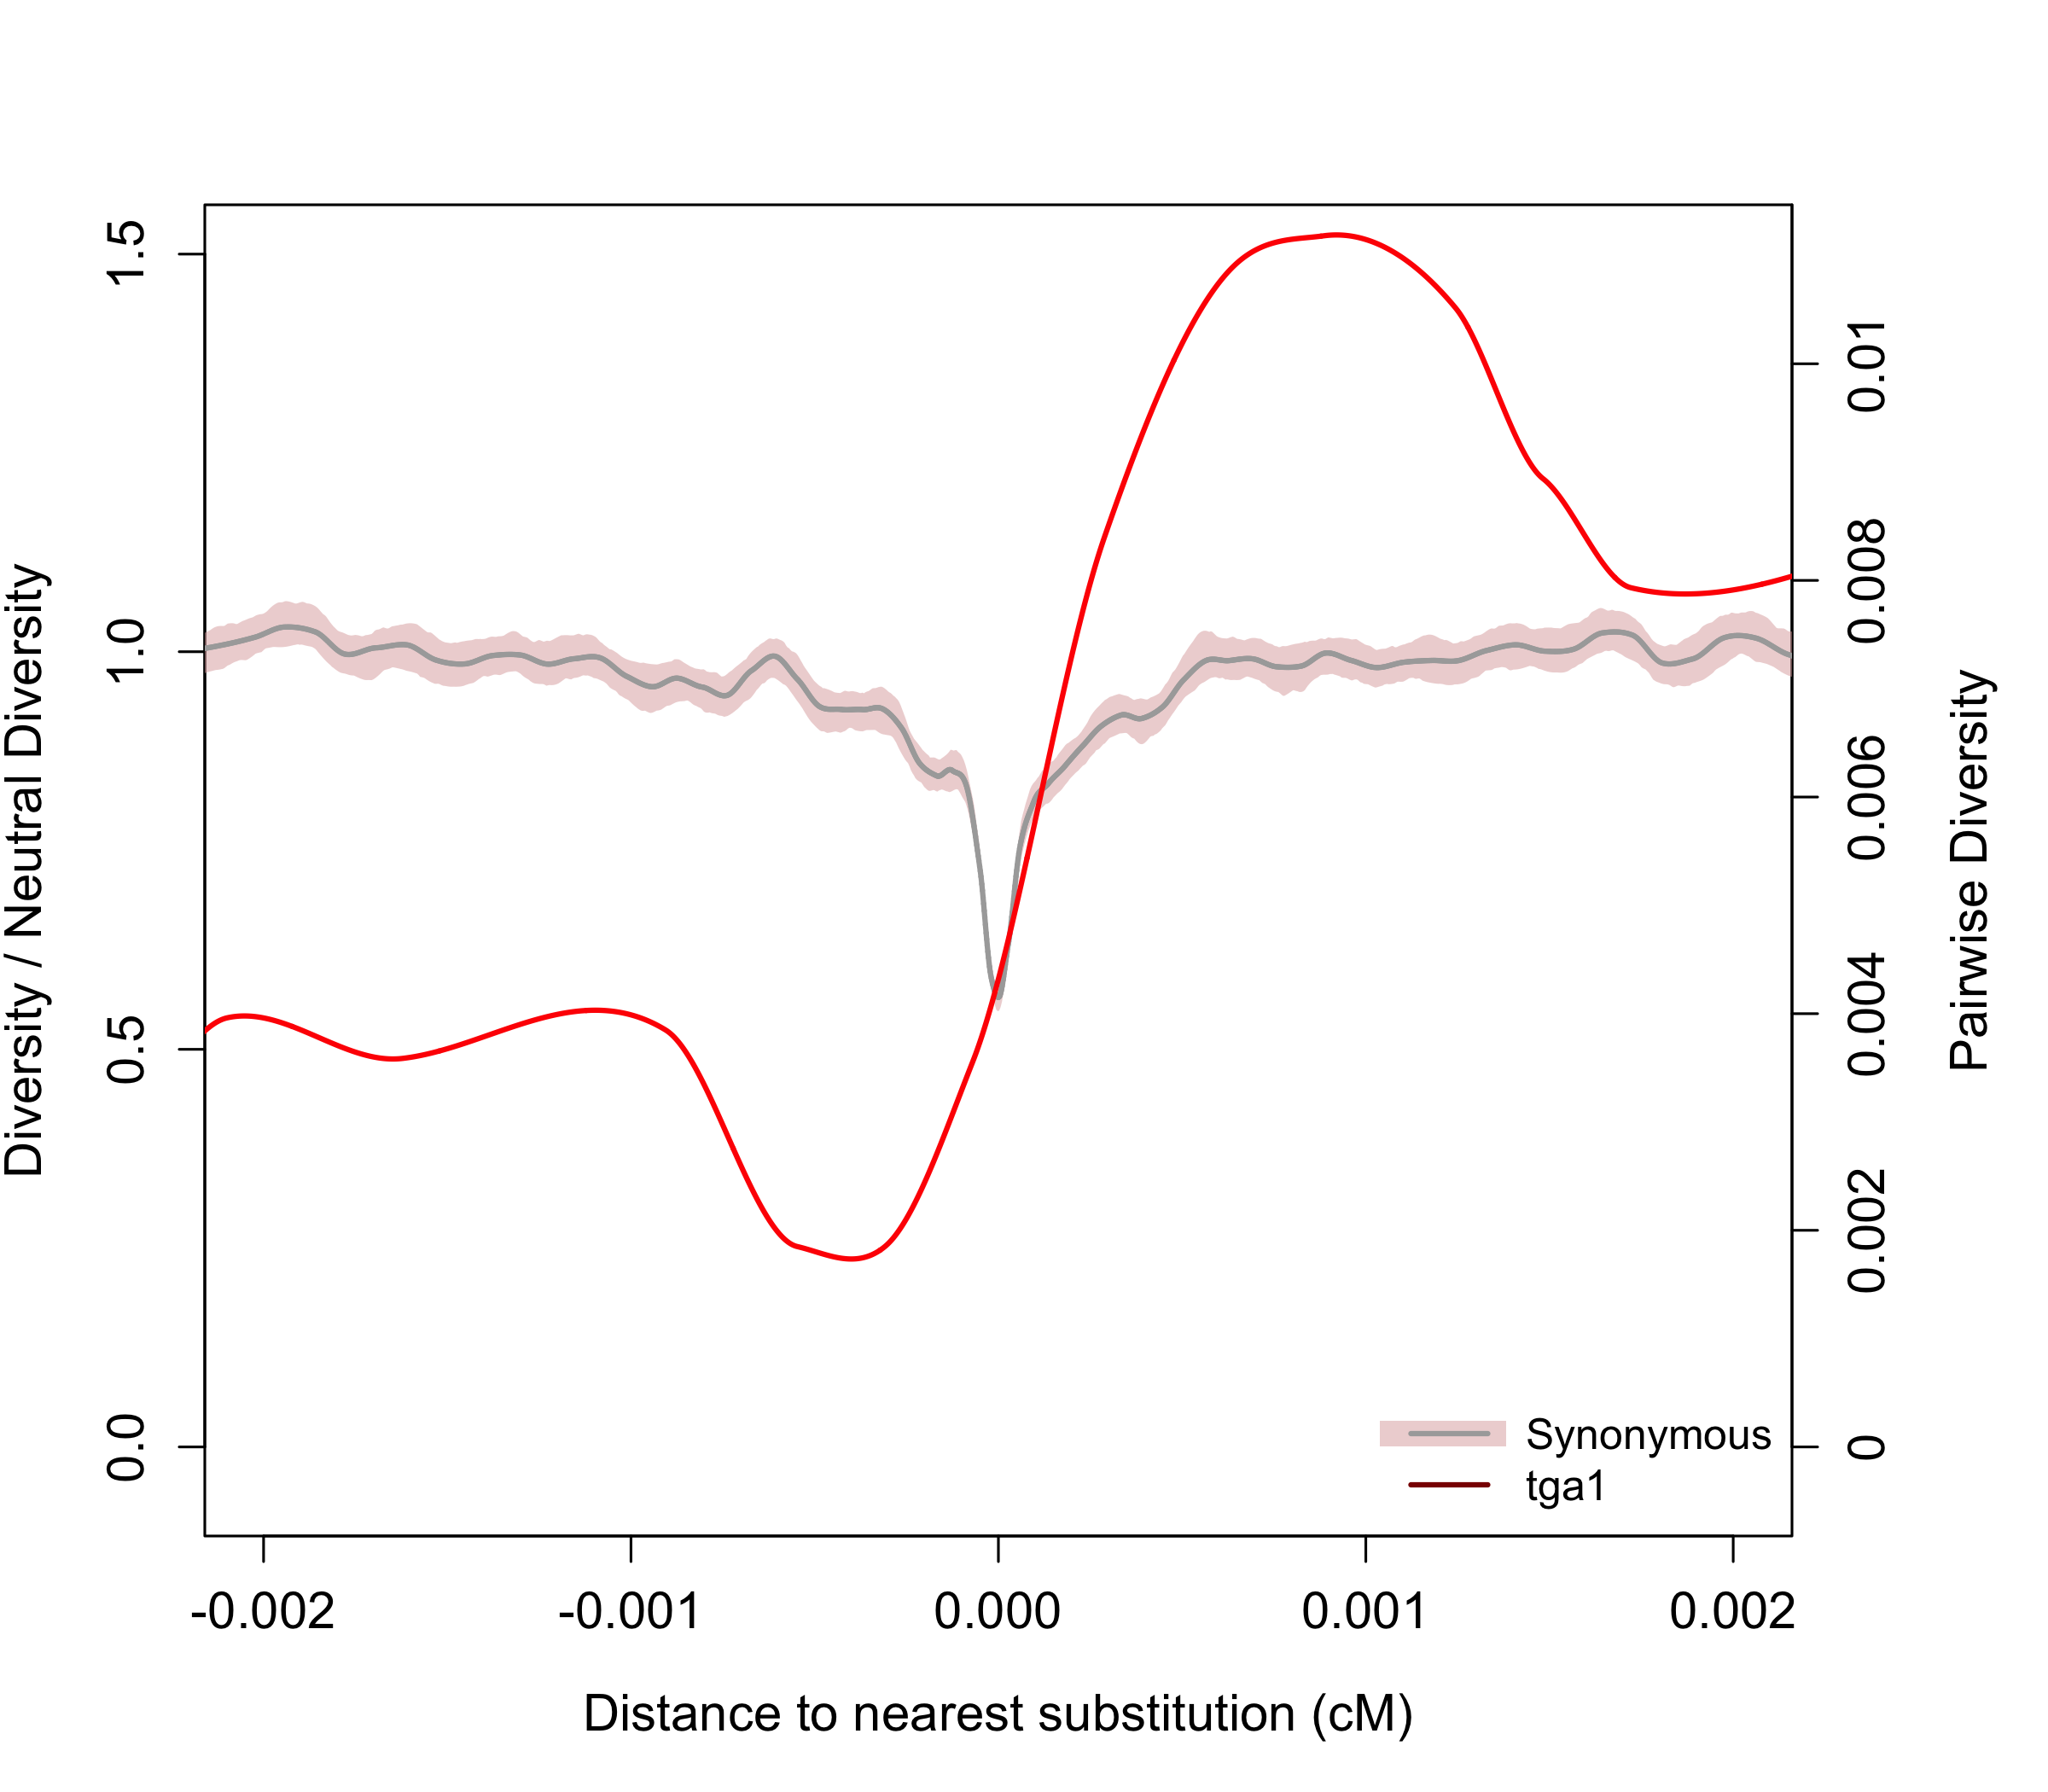
\includegraphics[width=.85\textwidth]{FigsAndFiles/plotDiversity_TvM_Folded2_Significance_tga1Supp_June.png} \\
    \end{center}
\caption{Diversity surrounding the causitive polymorphism at the \emph{tga1} locus is plotted. Since this is only one gene, the large amount of noise compared to our average plots is expected. However, notice that diversity precisely at the causitive polymorphism is reduced and a recovery of diversity is observed away from that site. \label{sFig:tga1}}
\end{figure}
\clearpage


\begin{figure}
  \begin{center}
    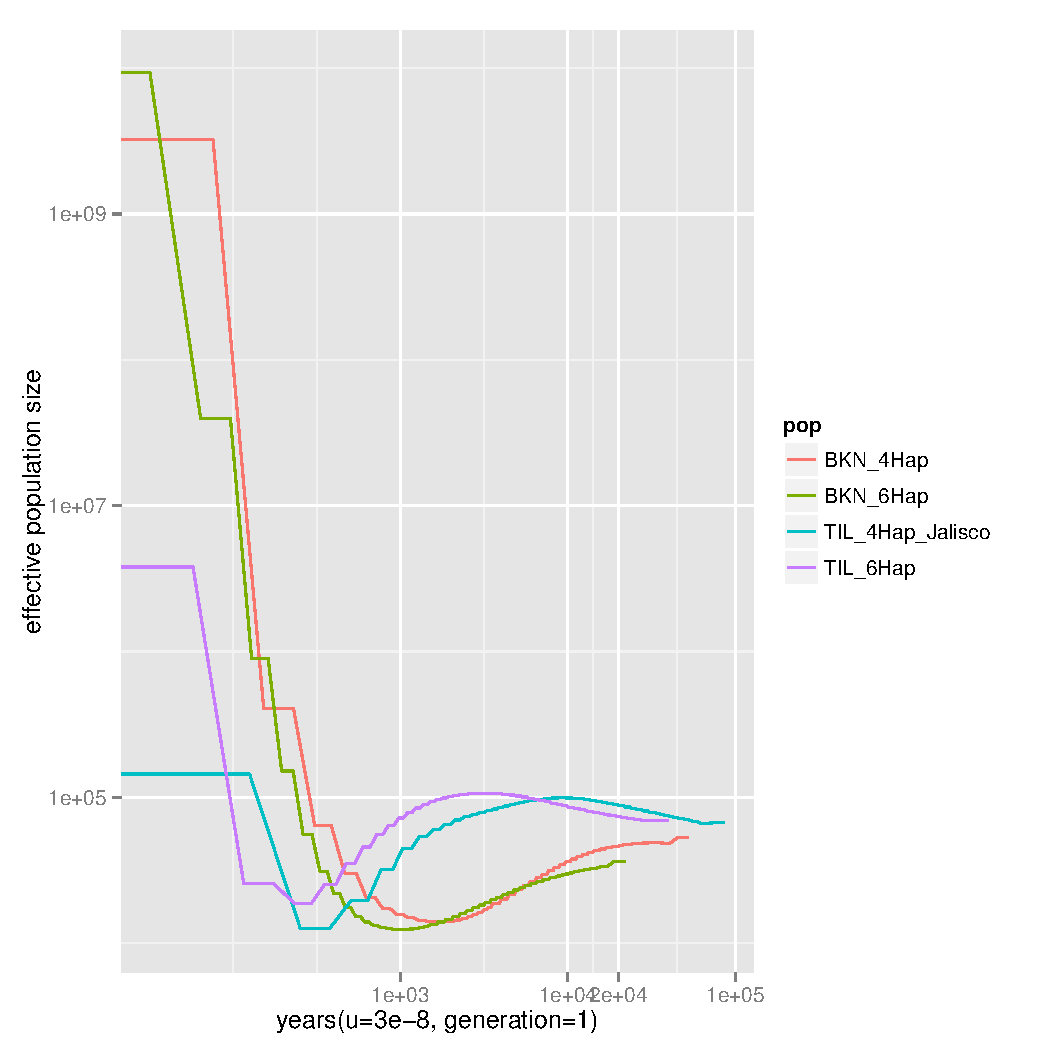
\includegraphics[width=.85\textwidth]{FigsAndFiles/BKN.TIL.msmc.pdf} \\
    \end{center}
\caption{\jri{need MSMC caption} \label{sFig:msmc}}
\end{figure}
\clearpage


\begin{figure}
  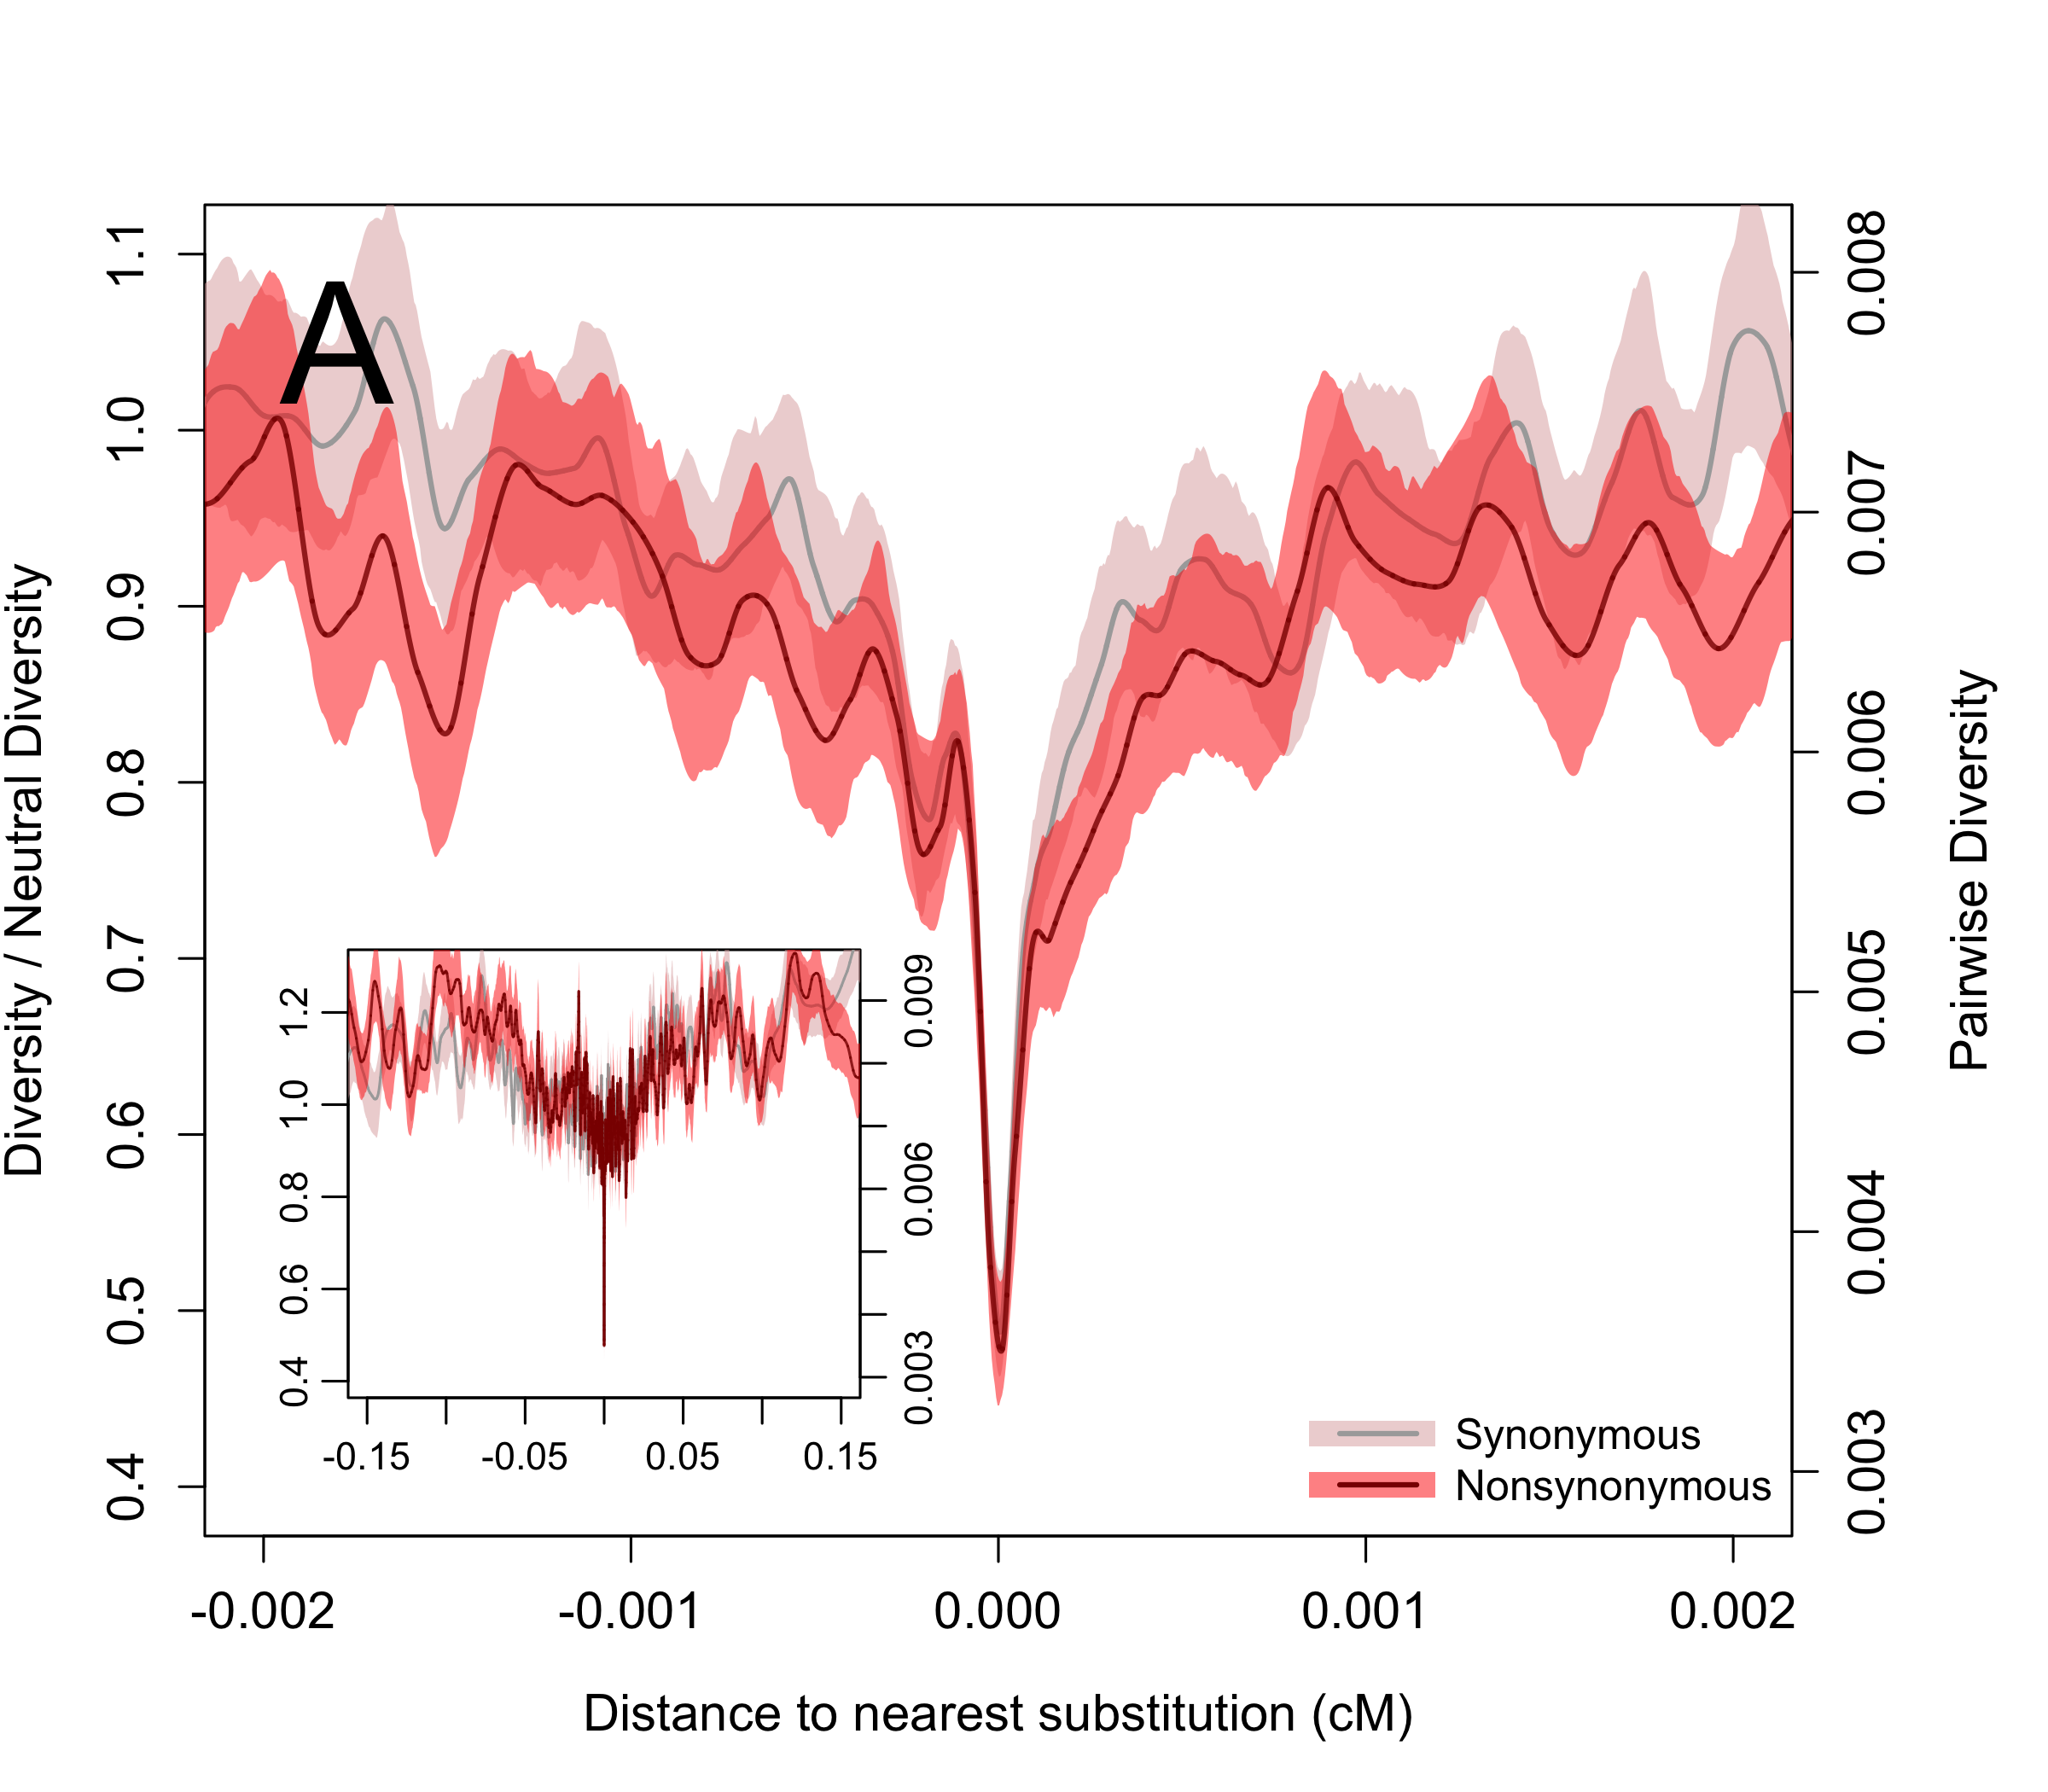
\includegraphics[width=.5\textwidth]{FigsAndFiles/plotDiversity_TvM_Conserved_Significance_June.png}
  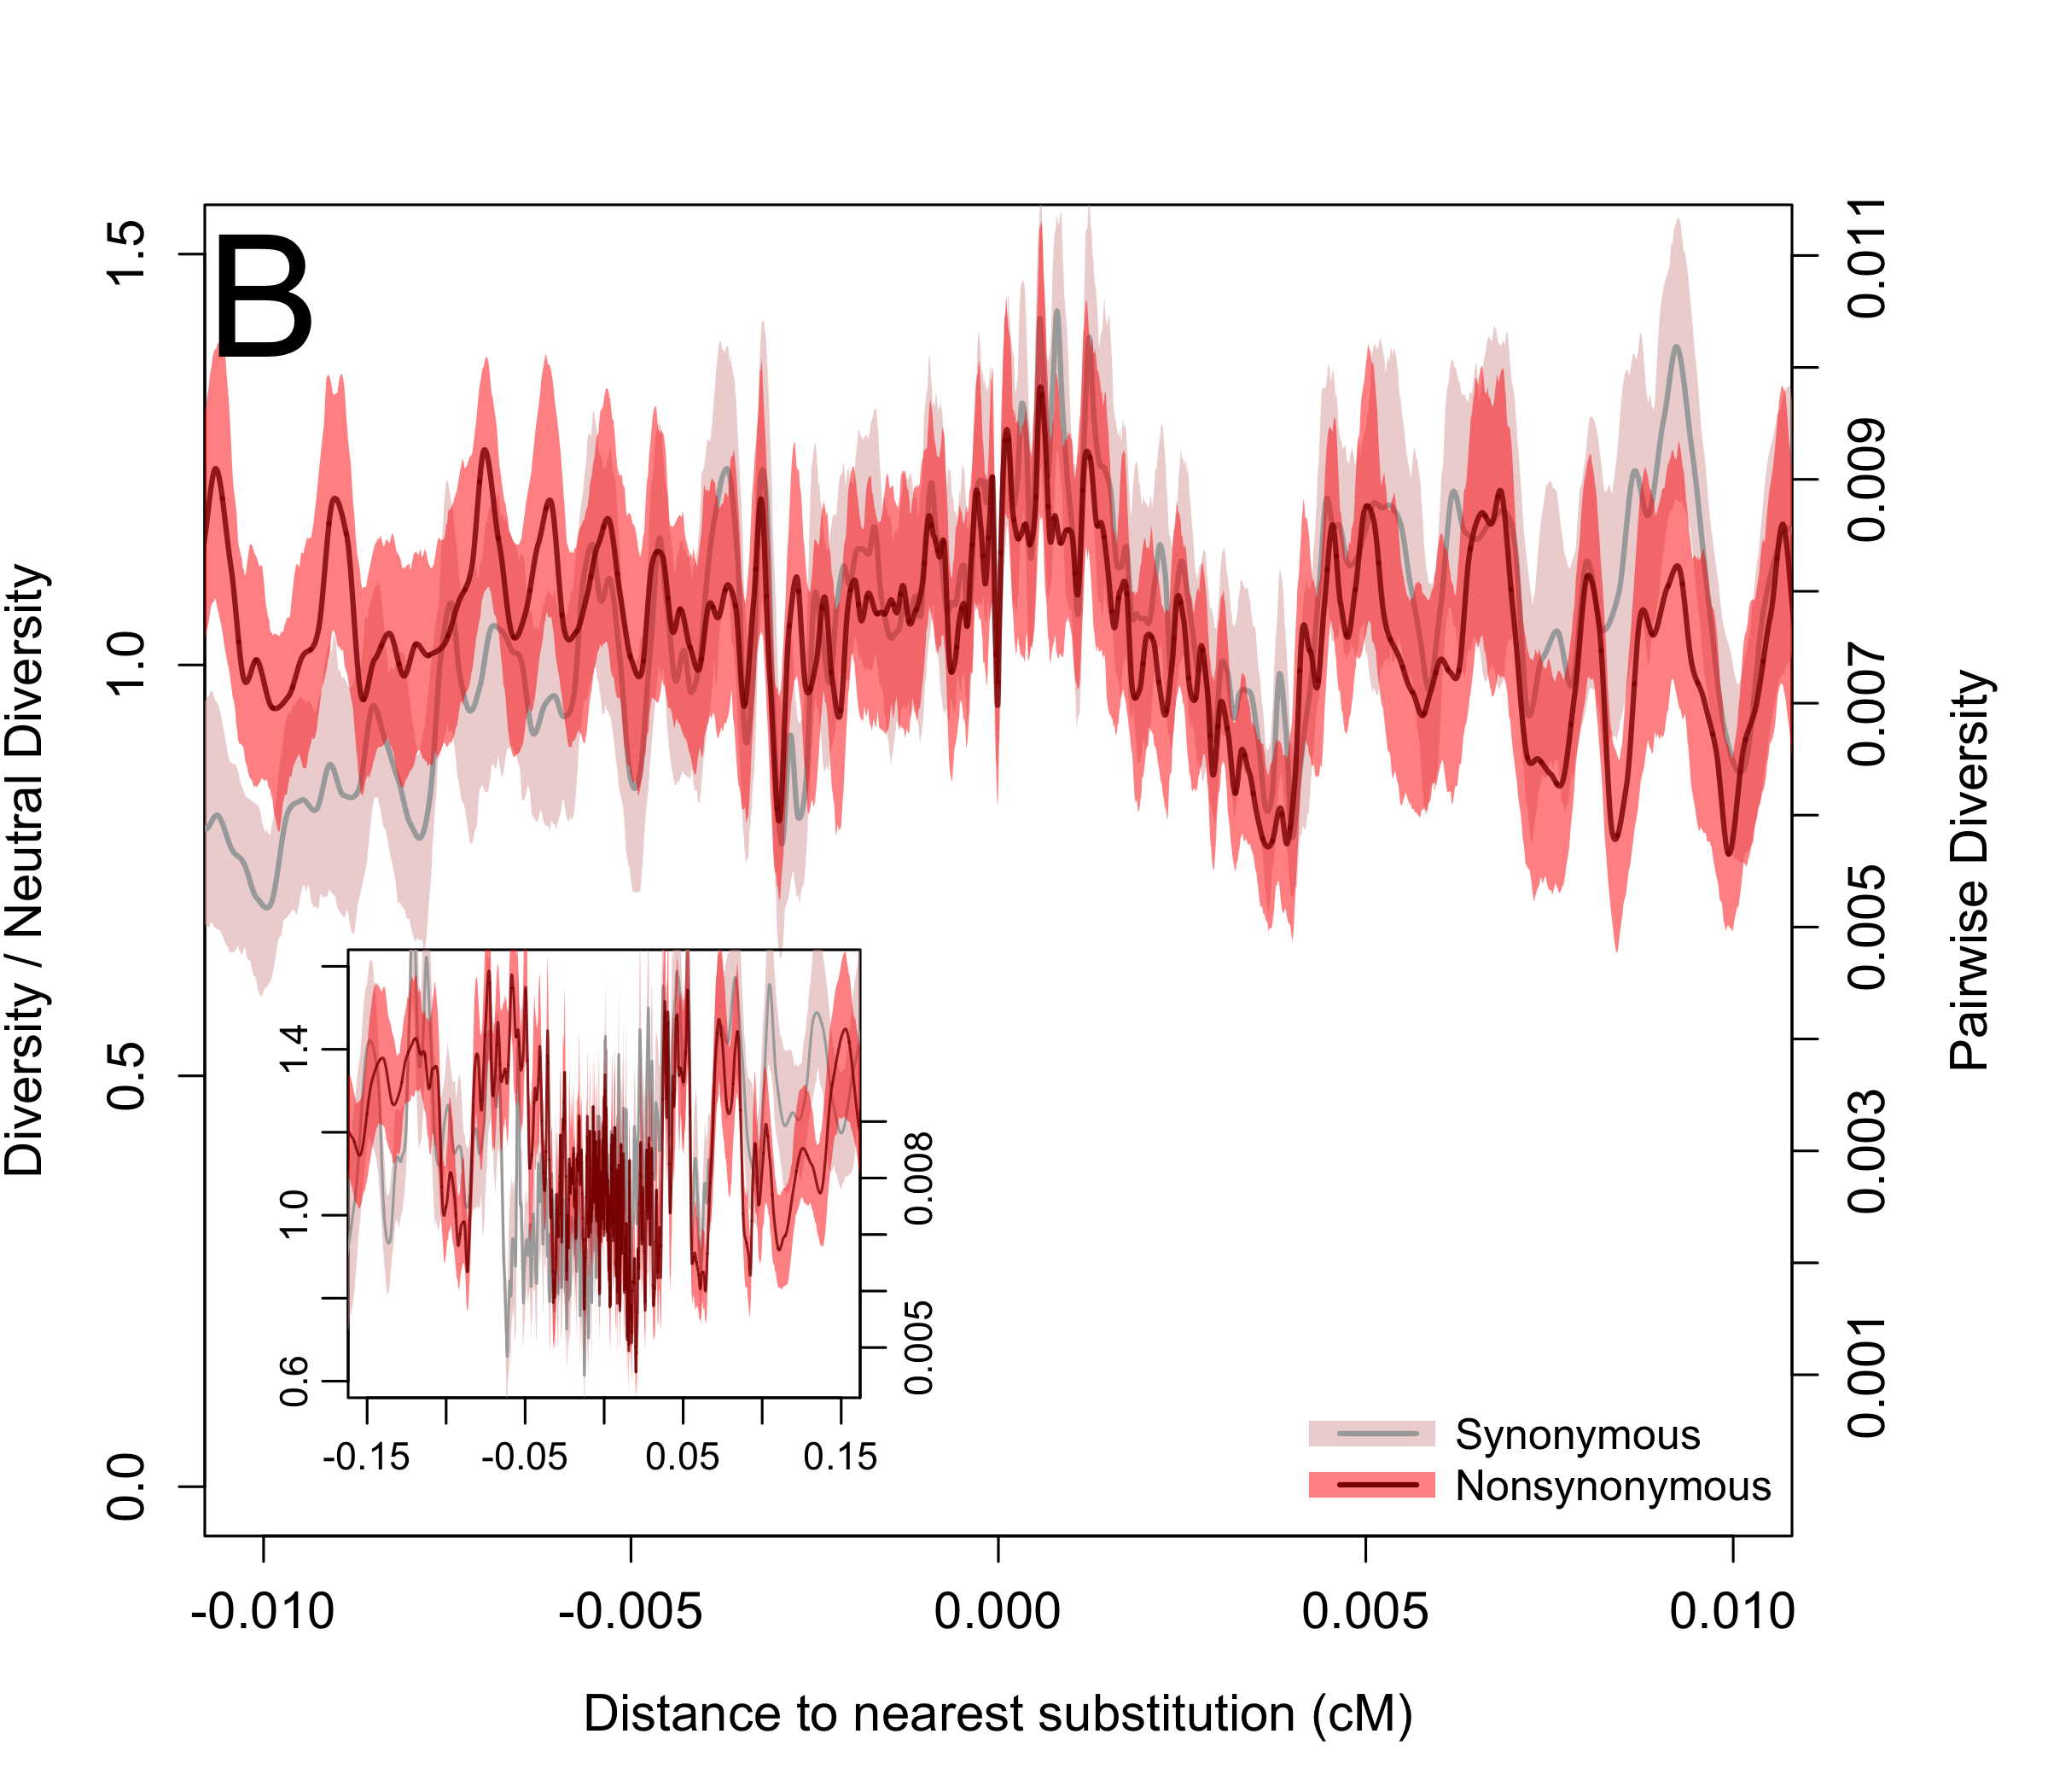
\includegraphics[width=.5\textwidth]{FigsAndFiles/plotDiversity_TvM_Unconserved_Significance_June.png}
\caption{ Pairwise diversity surrounding synonymous and nonsynonymous
  substitutions in maize at highly conserved (A) or unconserved (B) sites.  Bootstrap-based 95\% confidence intervals are depicted via shading. Inset plots depict a larger range on the x-axis. \label{sFig:consUncons}}
\end{figure}
\clearpage

\begin{figure}
  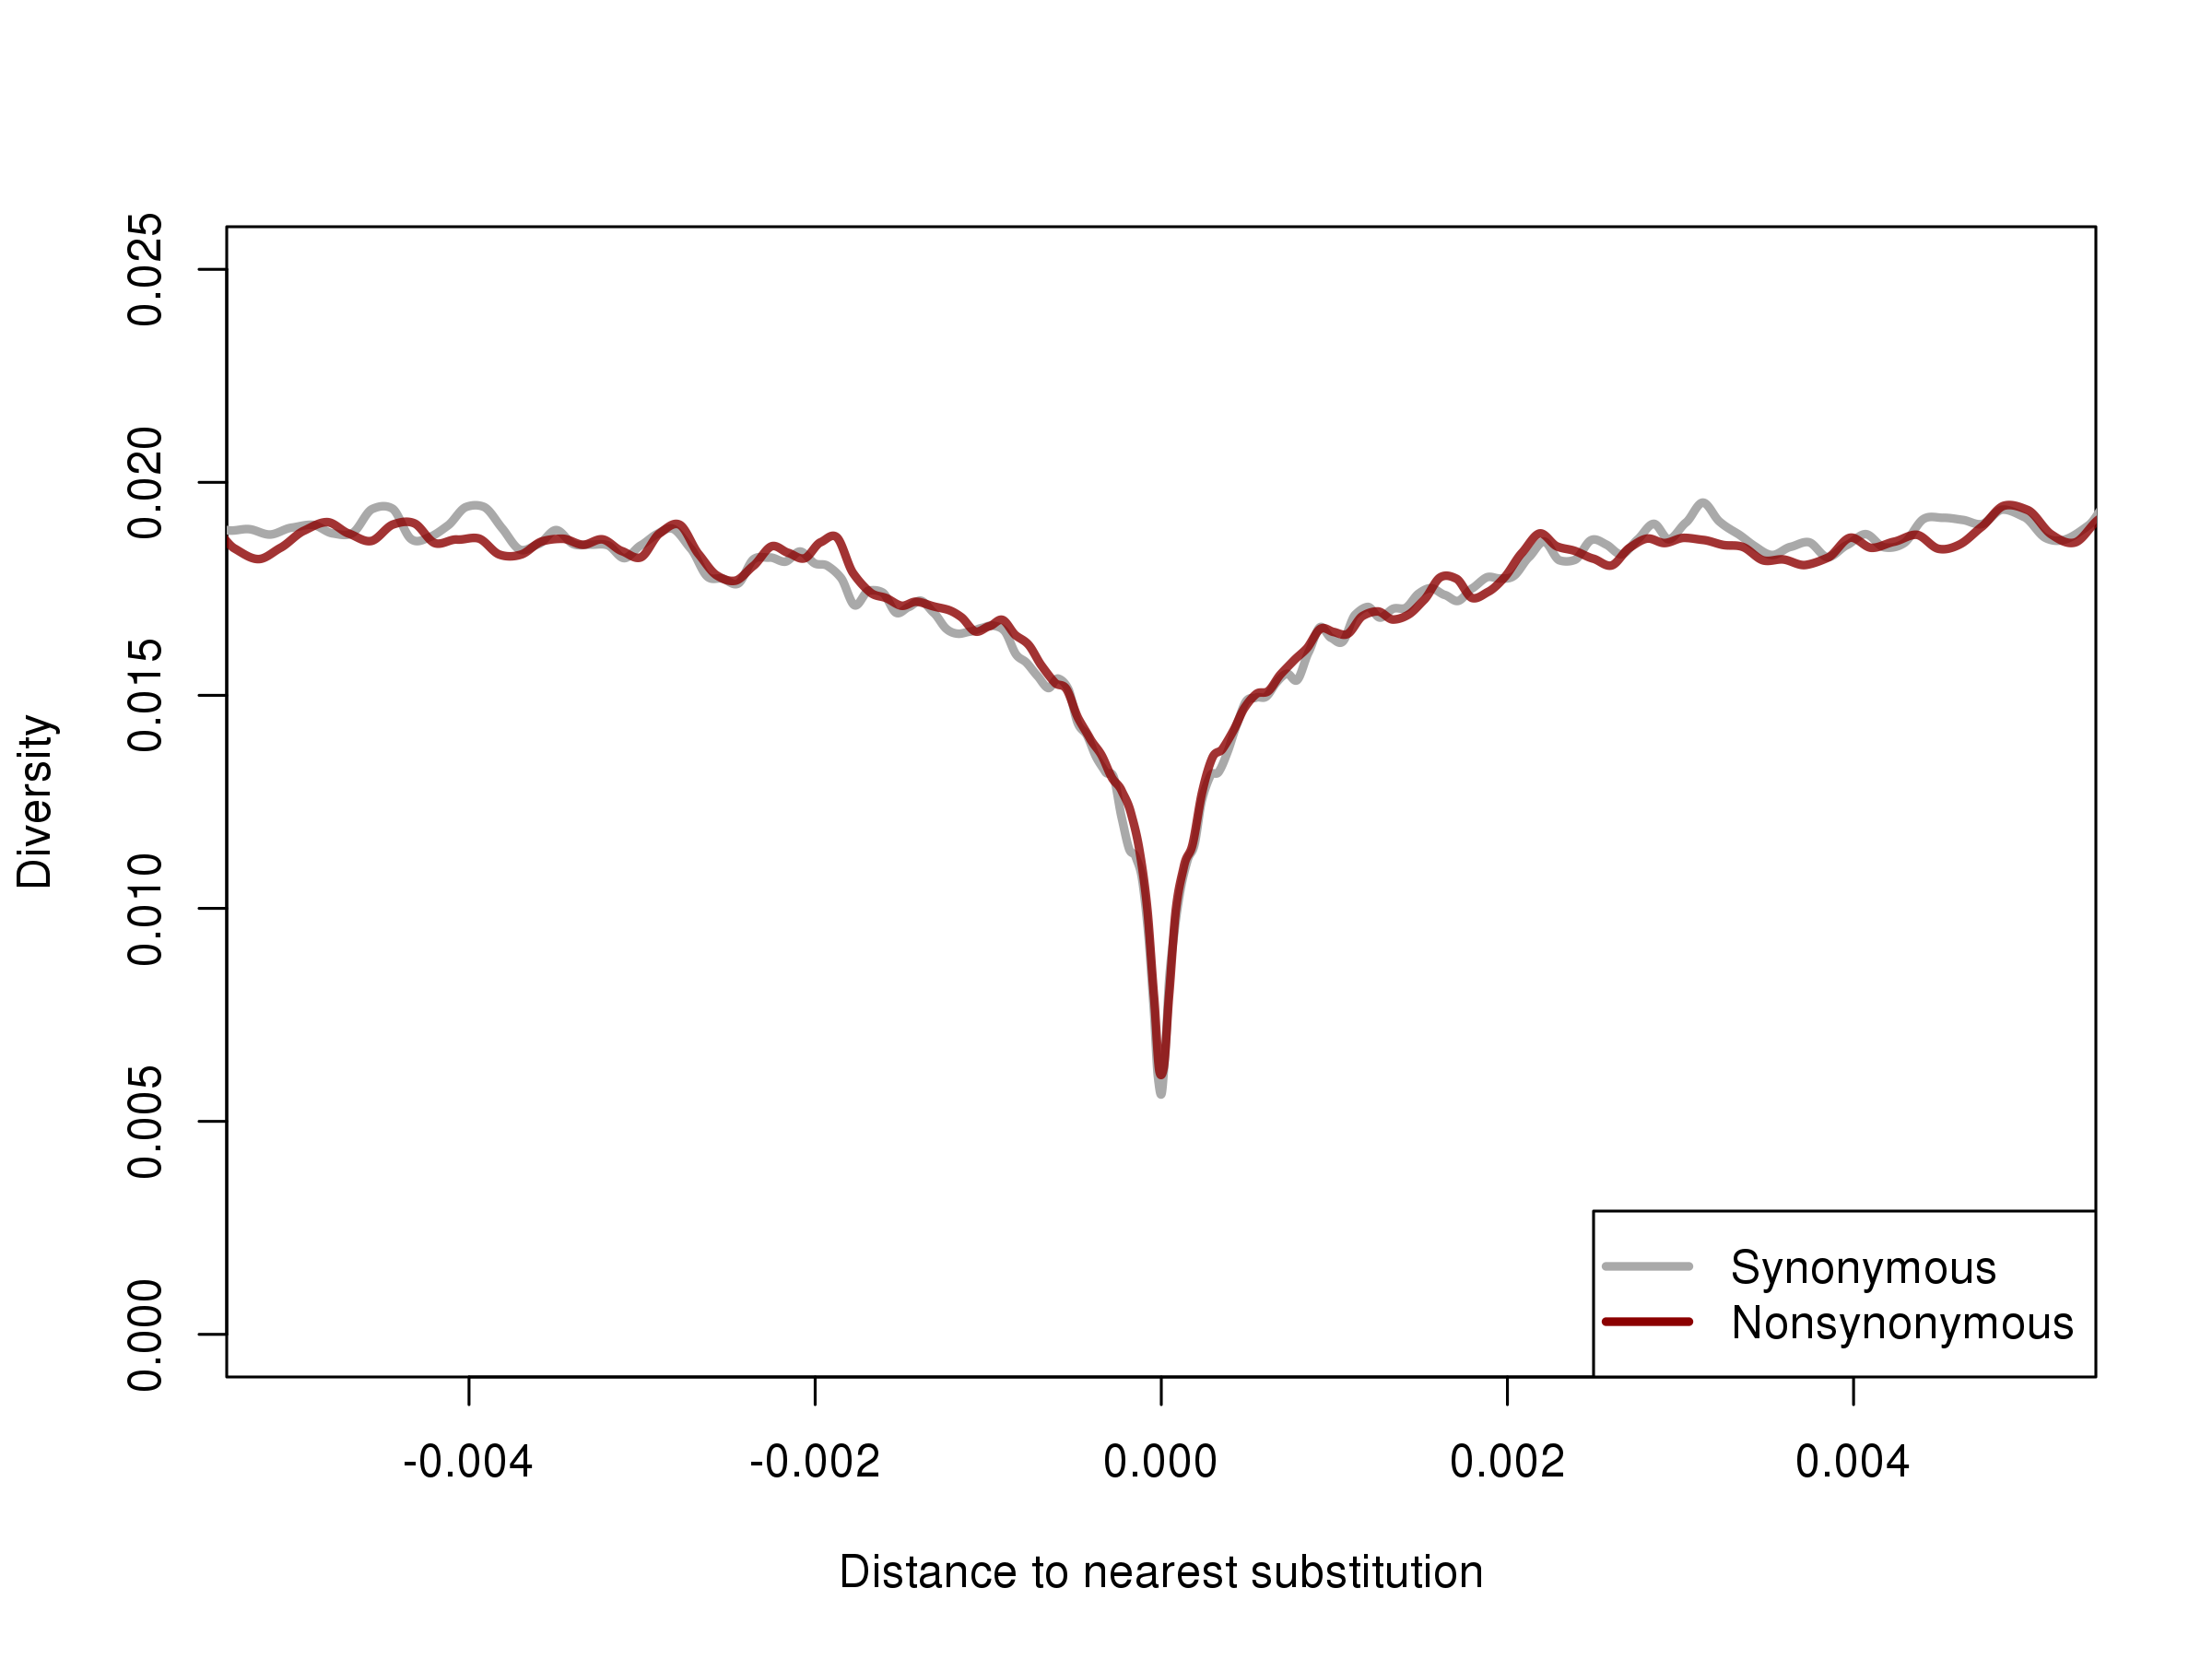
\includegraphics[width=\textwidth]{FigsAndFiles/plotDiversity_TvM_Singletons.png}
\caption{ Singleton diversity surrounding synonymous and nonsynonymous
  substitutions in maize. \label{sFig:singleton}}
\end{figure}
\clearpage


\begin{figure}
  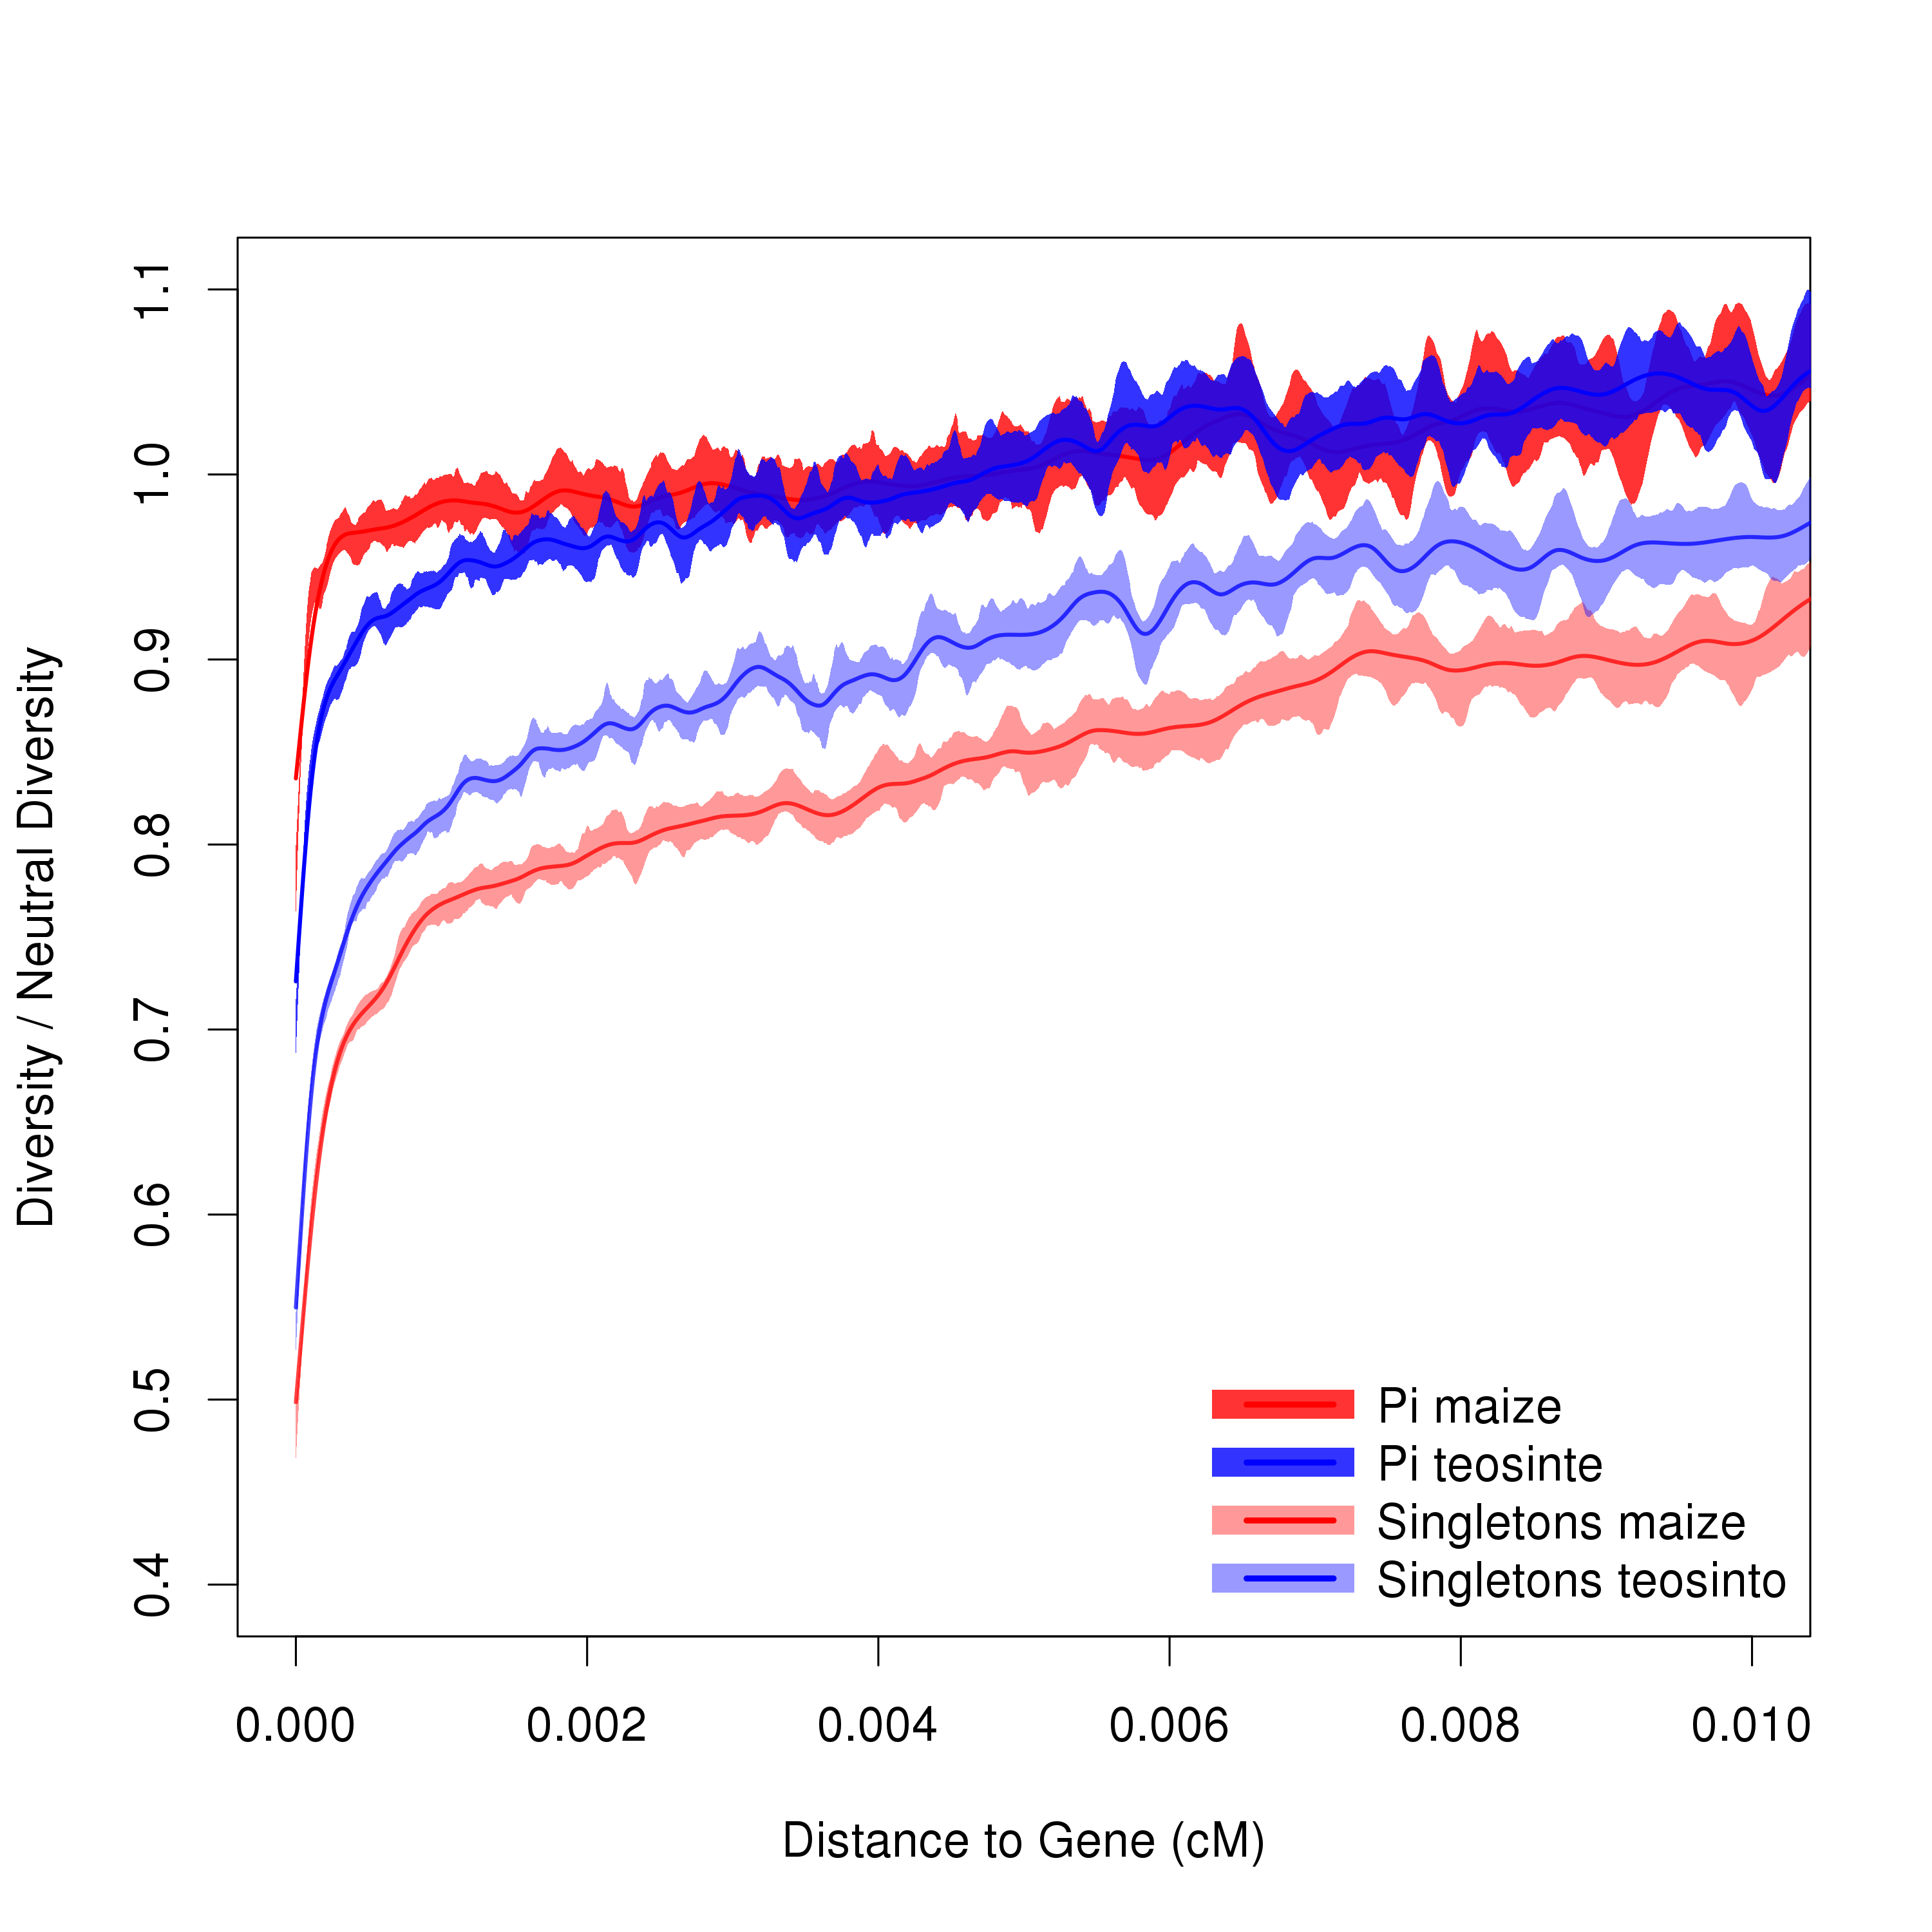
\includegraphics[width=\textwidth]{FigsAndFiles/distanceToGene_WithSignificance_Folded2_maizeAndTeoSingleVsPi.png}
\caption{ Relative diversity versus distance to nearest gene in maize and teosinte. Relative diversity is calculated by comparing to the mean diversity in all windows $\geq 0.02 cM$ from the nearest gene. Lines depict cubic smoothing splines with smoothing parameters chosen via generalized cross validation and shading depicts bootstrap-based 95\% confidence intervals.  \label{sFig:singletonPi}}
\end{figure}
\clearpage


\begin{figure}
  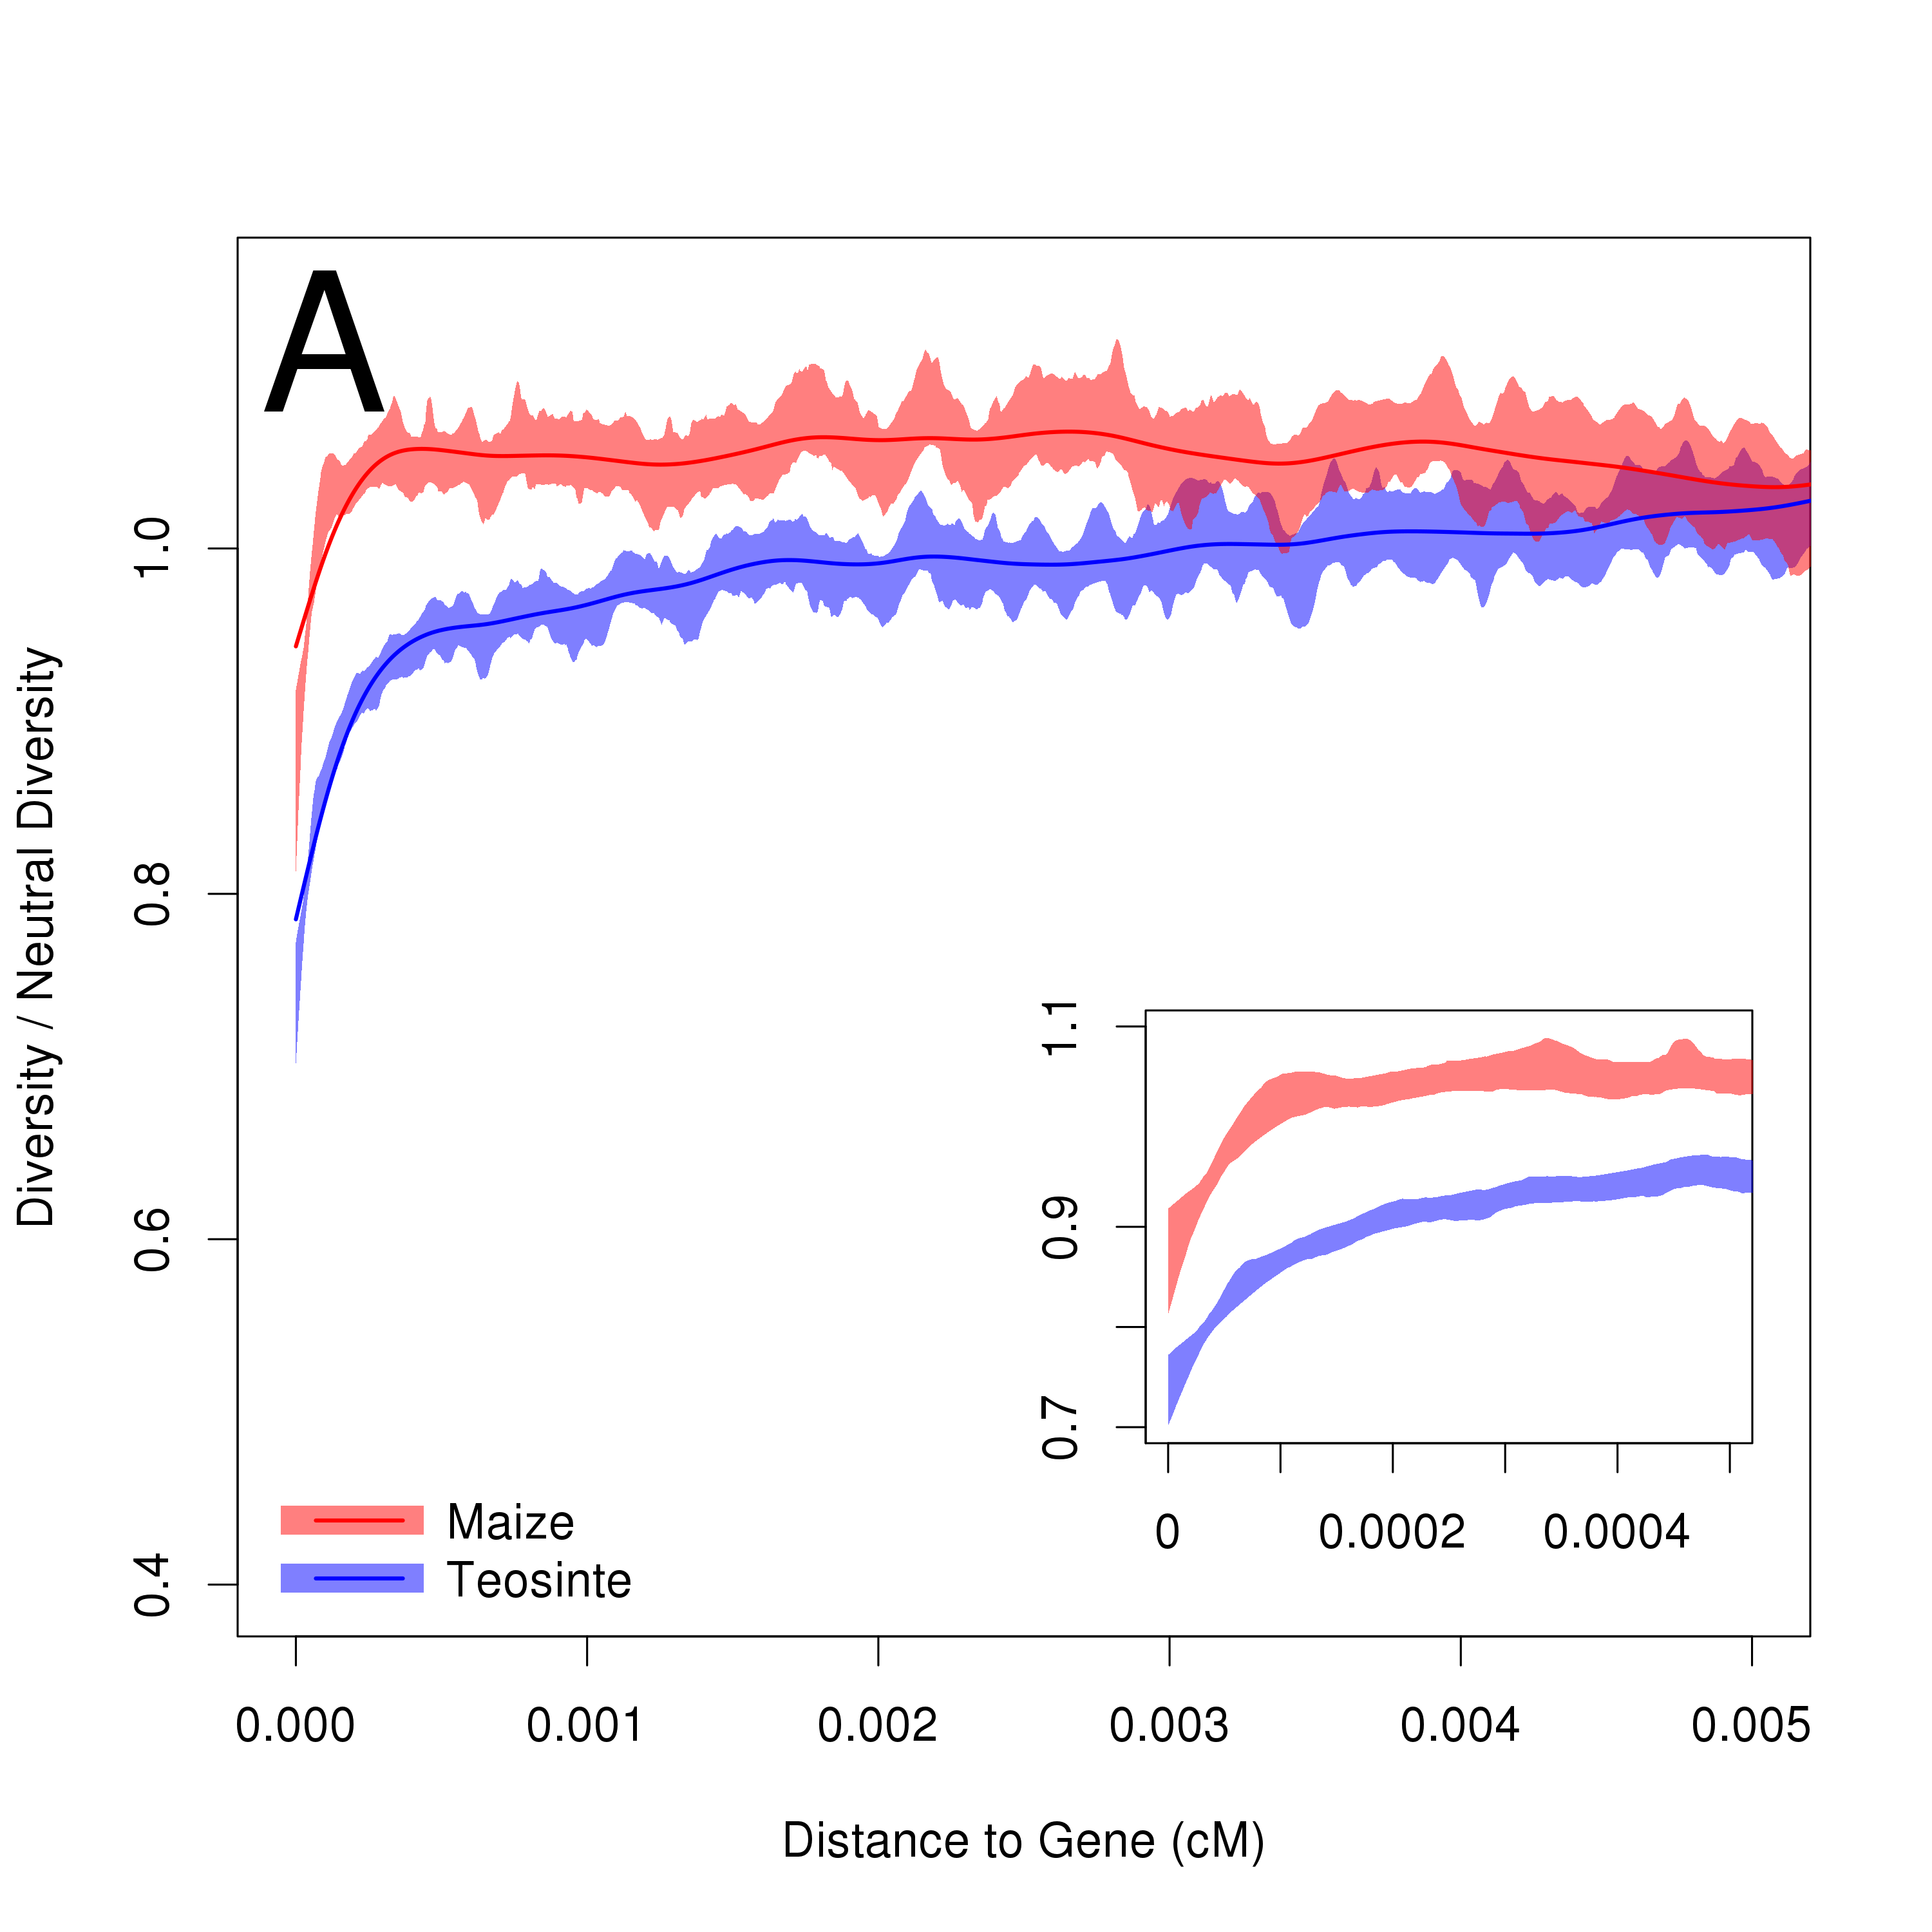
\includegraphics[width=.5\textwidth]{FigsAndFiles/distanceToGene_Unselected_manuscript.png}
    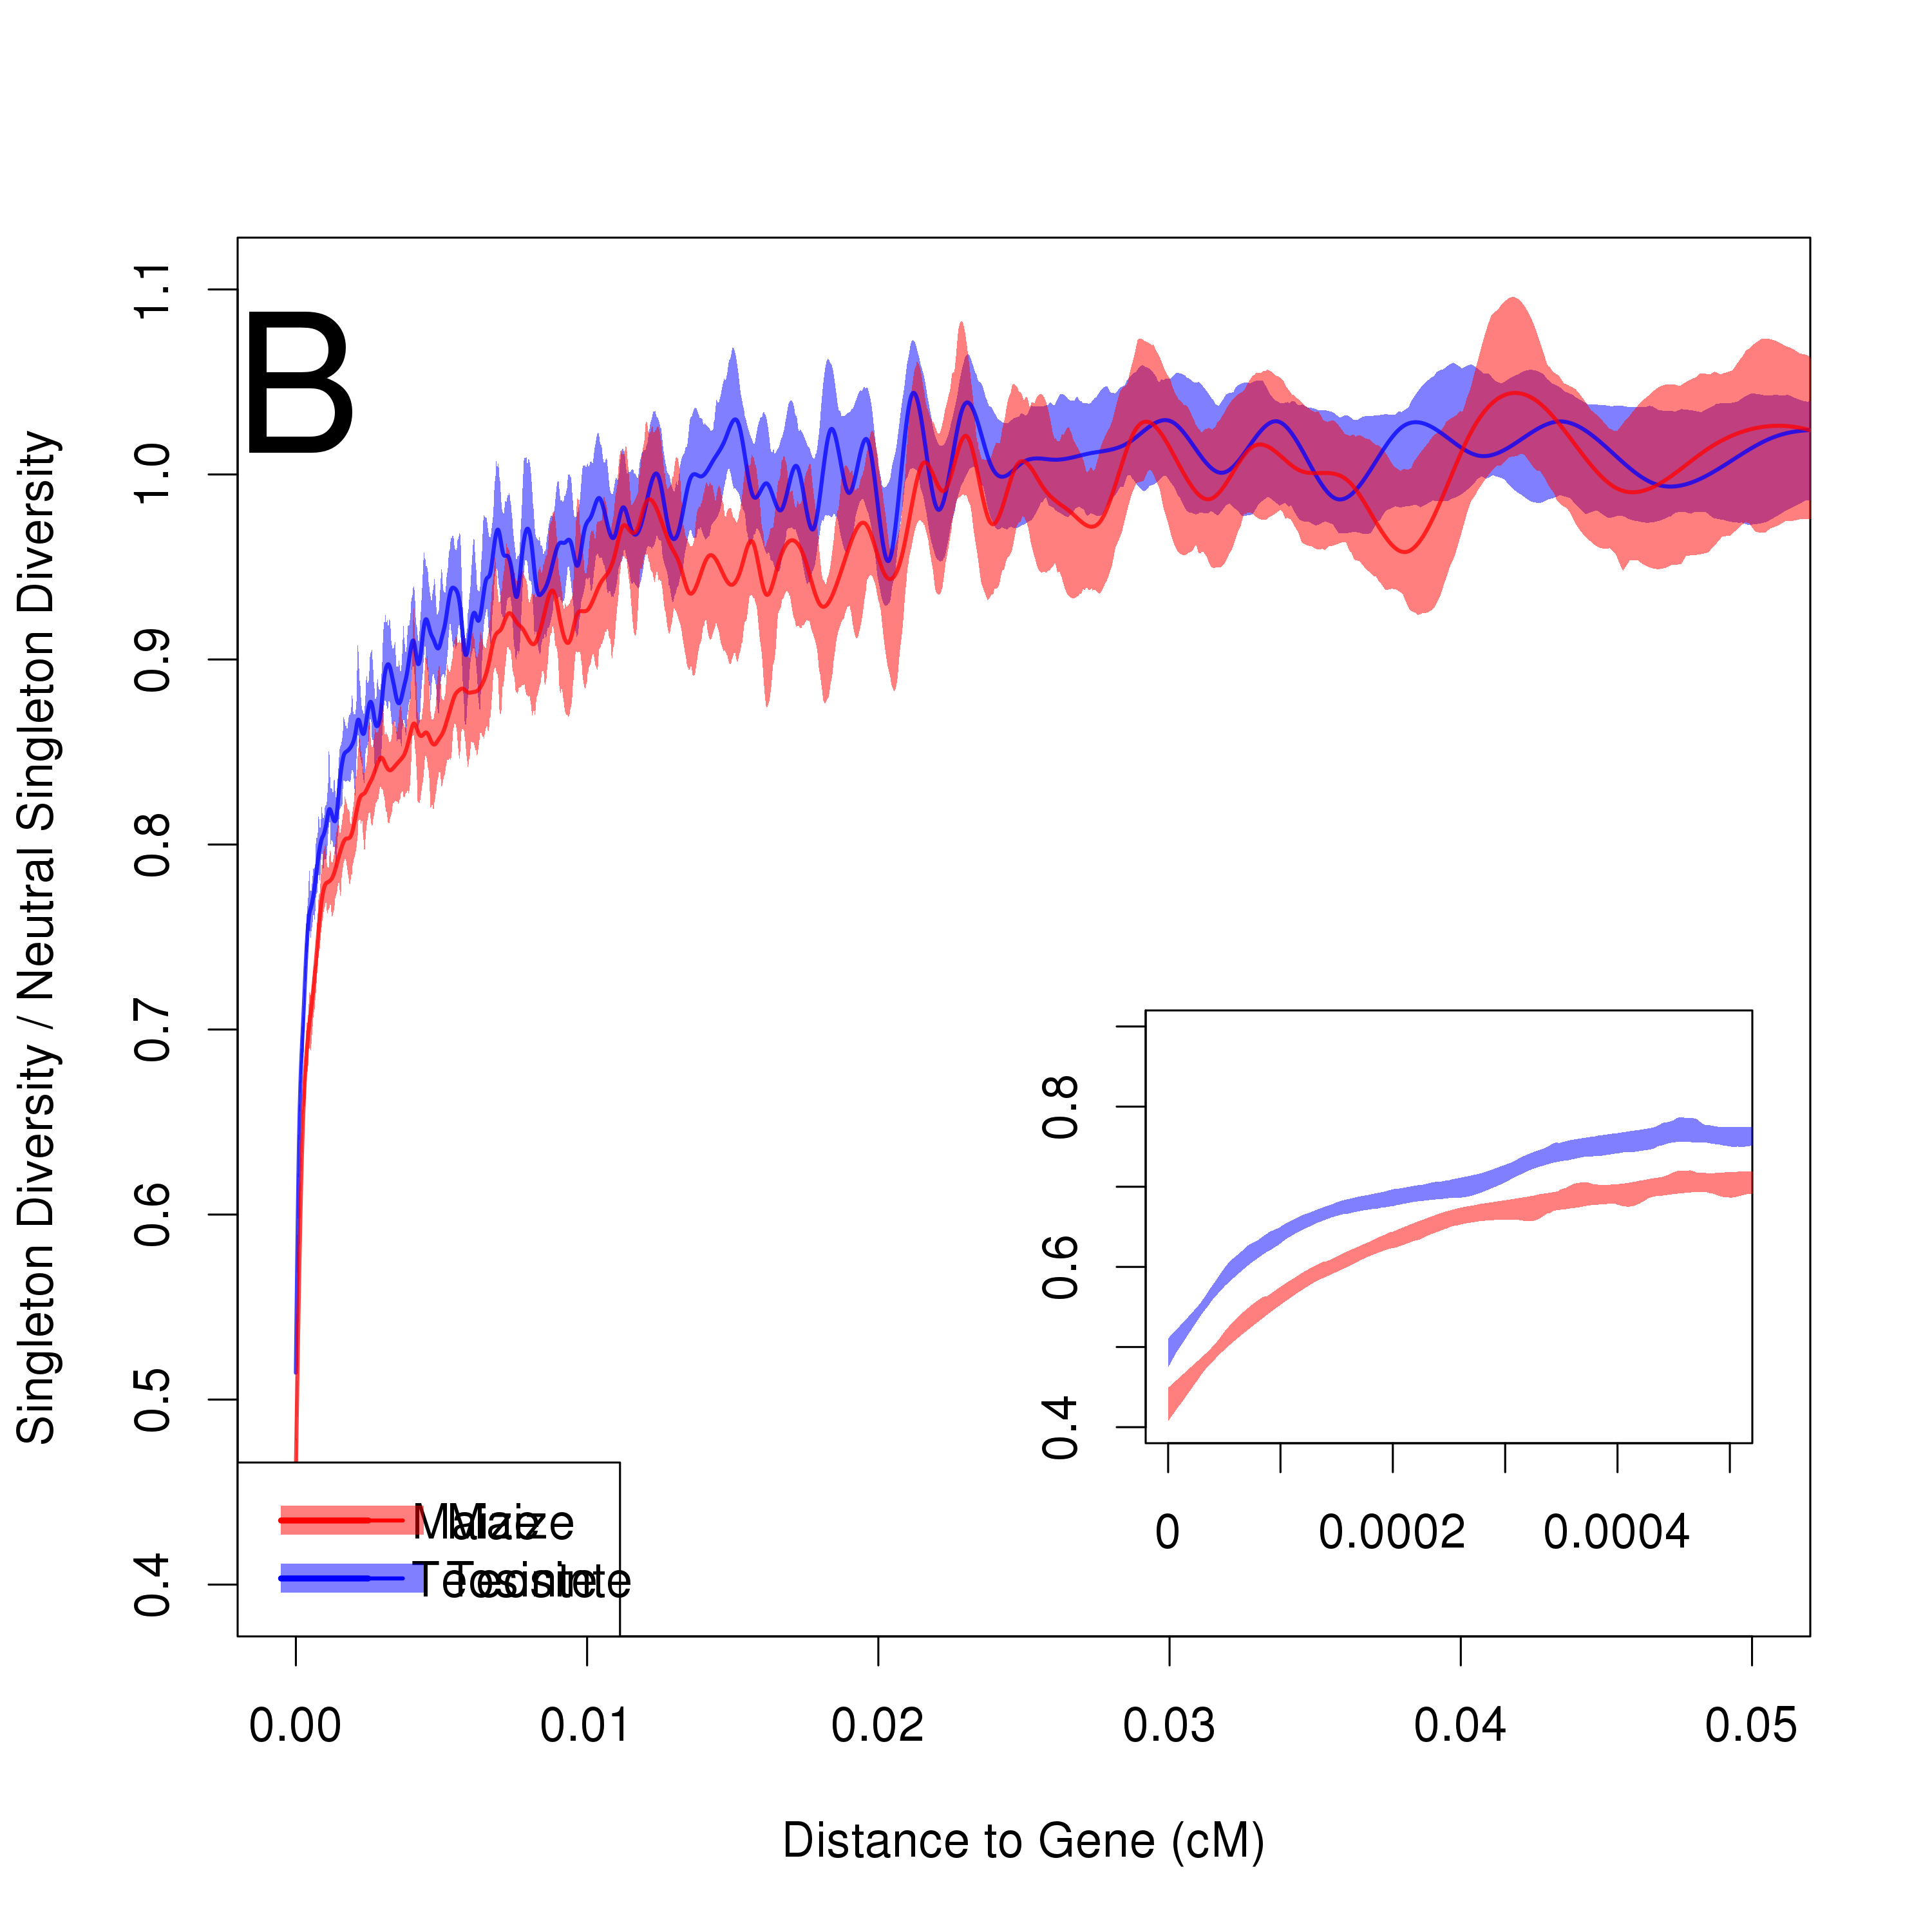
\includegraphics[width=.5\textwidth]{FigsAndFiles/distanceToGene_unselected_Singletons_manuscript.png}
\caption{ Relative level of diversity versus distance to the nearest gene, in maize and teosinte, based on only sites that do not show evidence of hard or soft sweeps according to H12. Two measures of diversity were investigated. {\bf A} displays pairwise diversity,
which is most influenced by intermediate frequency alleles and therefore depicts more ancient evolutionary patterns, and {\bf B} depicts singleton diversity, influenced by rare alleles and thus depicting evolutionary patterns in the recent past. Bootstrap-based 95\% confidence intervals are depicted via shading. Inset plots depict a smaller range on the x-axis. \label{sFig:H12}}
\end{figure}
\clearpage


\begin{figure}
  \begin{center}
  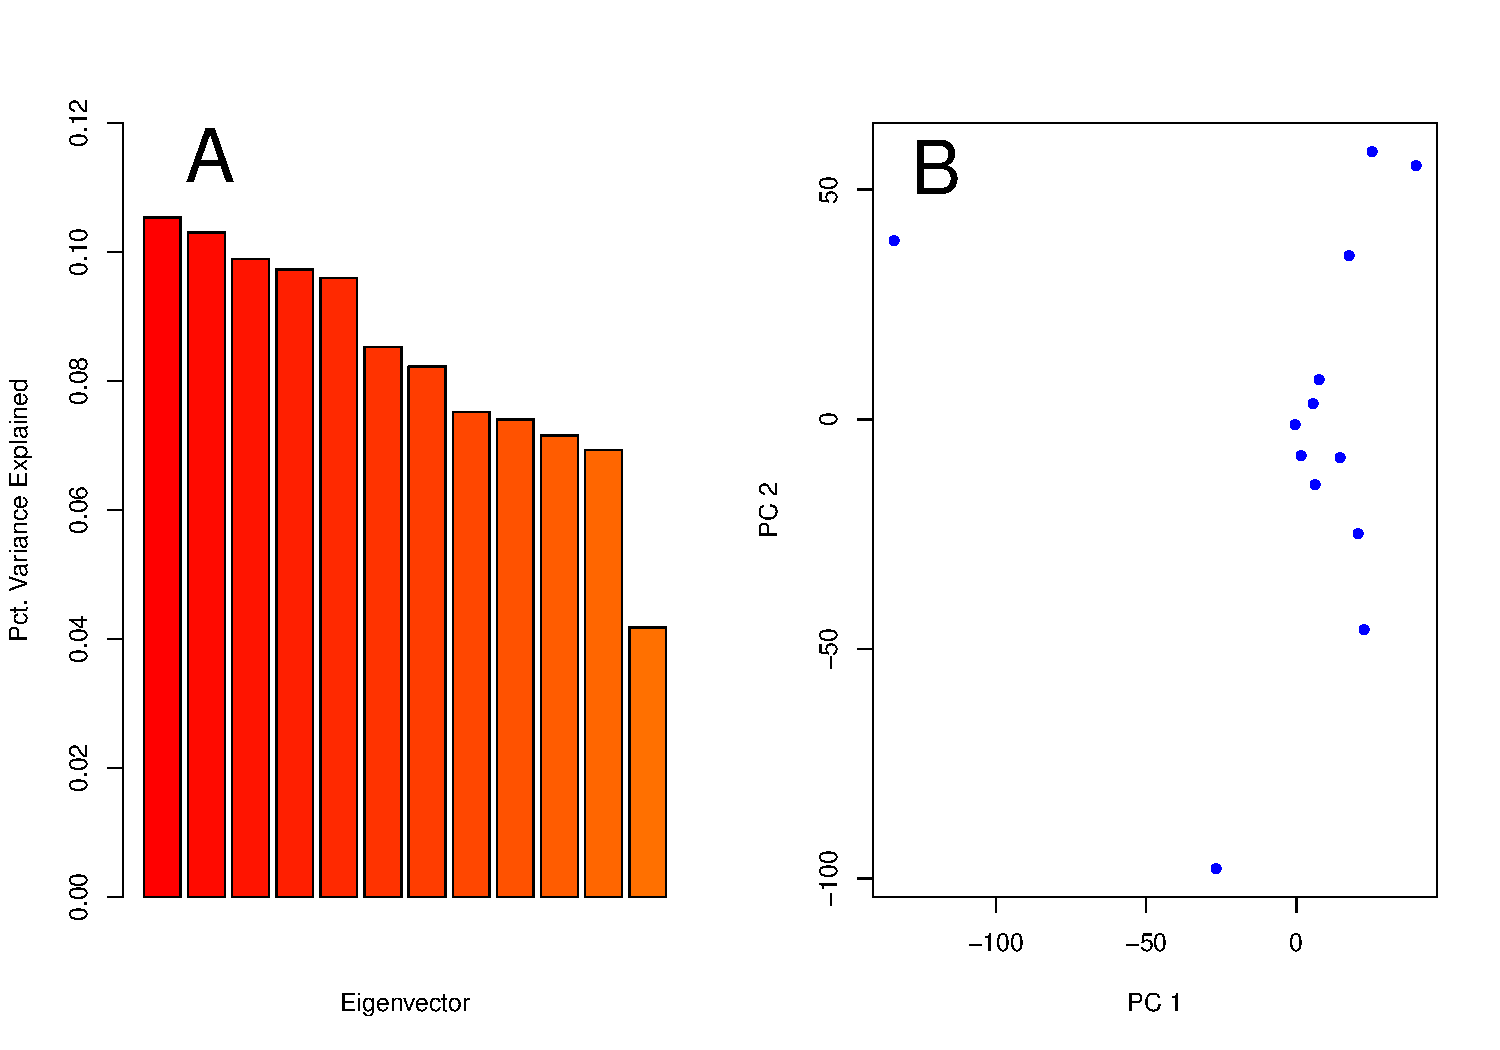
\includegraphics[width=.75\textwidth]{FigsAndFiles/tilPCA_aug.pdf}\\
  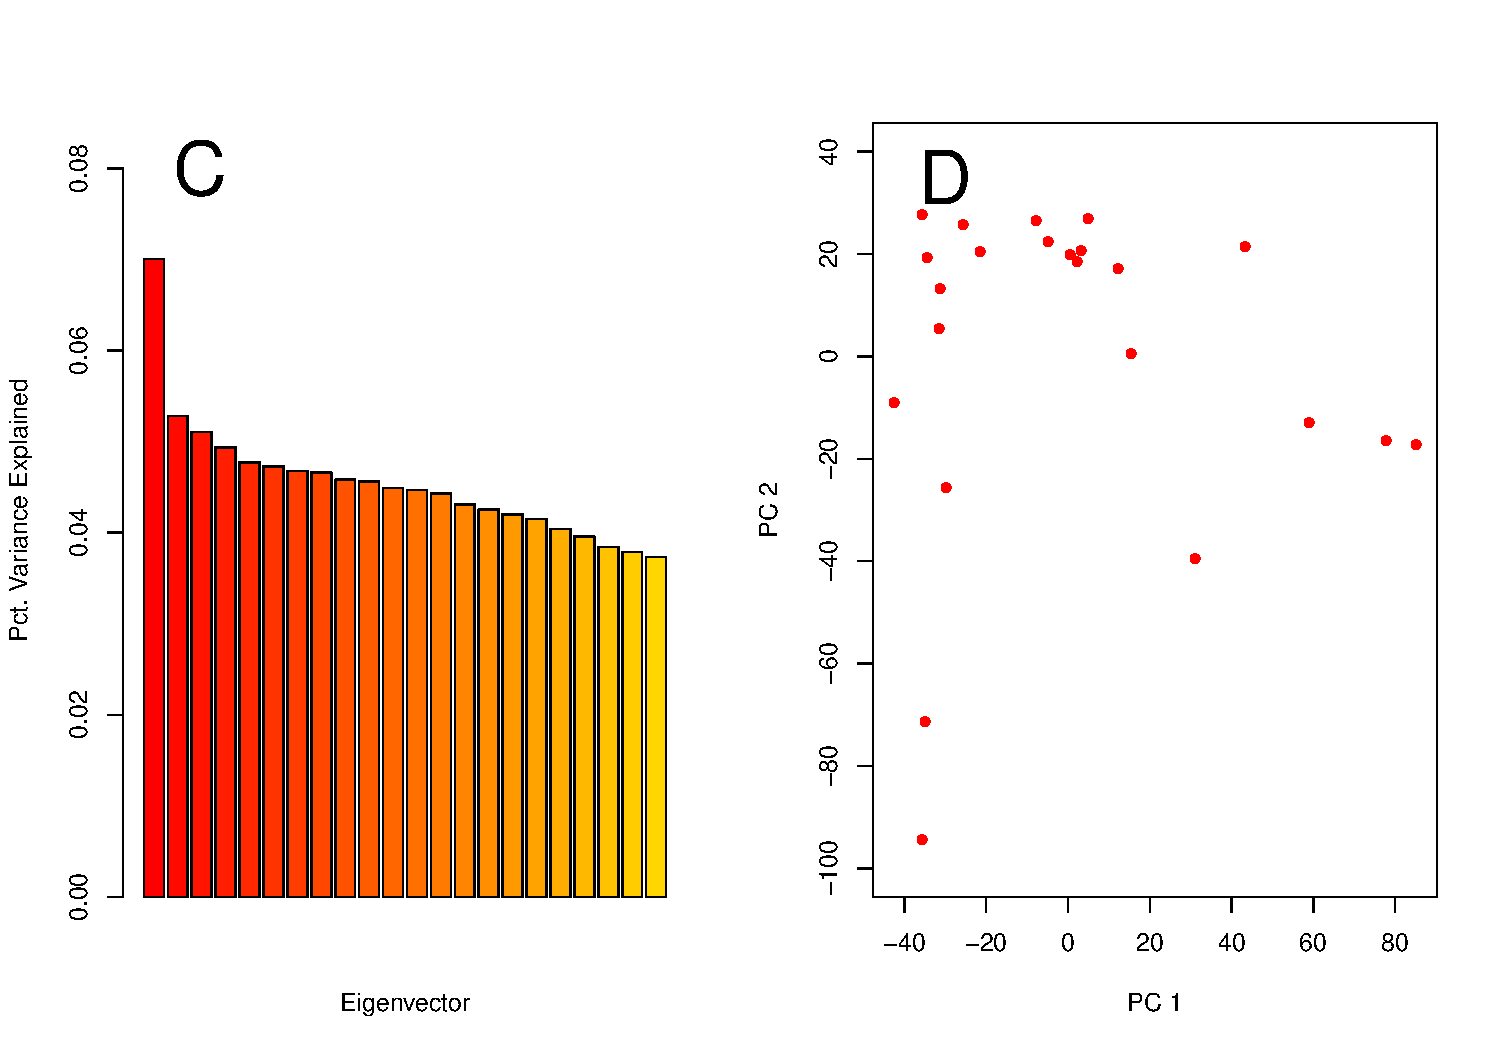
\includegraphics[width=.75\textwidth]{FigsAndFiles/bknPCA_aug.pdf}\\
  \end{center}
  \caption{Principal component analysis of teosinte and maize individuals to ensure that no close relatives were inadvertantly included in our study. Plots are based on a random sample of 10,000 SNPs. {\bf A:} Percentage of total variance explained by each principal component for teosinte. {\bf B:} PC1 vs PC2 for all 13 teosinte individuals. {\bf C:} Percentage of total variance explained by each principal component for maize. {\bf D:} PC1 vs PC2 for all 23 maize individuals. \label{sFig:PCA}}
\end{figure}
\clearpage


\begin{figure}
%  \begin{center}
  \begin{tabular}{c|c}
    \bf Maize & \bf Teosinte \\ \hline \hline
    BKN009 &  TIL01 \\
    BKN010 & TIL02 \\
    BKN011 & TIL03 \\
    BKN014 & TIL04-TIP454 \\
    BKN015 & TIL07 \\
    BKN016 & TIL09 \\
    BKN017 & TIL10 \\
    BKN018 & TIL11 \\
    BKN019 & TIL12 \\
    BKN020 & TIL14-TIP498 \\
    BKN022 & TIL15 \\
    BKN023 & TIL16 \\
    BKN025 & TIL17 \\
    BKN026 & \\
    BKN027 & \\
    BKN029 & \\
    BKN030 & \\
    BKN031 & \\
    BKN032 & \\
    BKN033 & \\
    BKN034 & \\
    BKN035 & \\
    BKN040 & \\
  \end{tabular} 
%  \end{center}
  \caption{ A list of maize and teosinte individuals included in this study. Sequencing and details were previously described by \jri{cite chia and lemmon}   \label{sTab:list} }
\end{figure}
\clearpage

\begin{figure}
  \def\arraystretch{2}
%  \begin{center}
  \begin{tabular}{l|c|c|c}
    \bf Parameter & \bf Initial value & \bf Upper bound & \bf Lower bound\\ \hline 
    $\frac{N_b}{N_a}$ & 0.02 & $1\times10^{-7}$ & 2 \\ 
    $\frac{N_{m}}{N_a}$ & 3 & $1\times10^{-7}$ & 200 \\
    $\frac{T_b}{2N_a}$ & 0.04 & 0  & 1 \\ 
    $\frac{M_{mt}}{N_a}$ & $1\times10^{-10}$ & $1\times10^{-7}$ & 0.001 \\
    $\frac{M_{tm}}{N_a}$ & $1\times10^{-10}$ & $1\times10^{-7}$ & 0.001 \\
  \end{tabular} 
%  \end{center}
  \caption{ Parameters, initial values, and boundaries used for model-fitting with $\delta\alpha\delta{i}$. Parameters are shown in the units utilized by $\delta\alpha\delta{i}$, although in the text simplified units are reported.   \label{sTab:dadi} }
    \def\arraystretch{1} % undo stretching
\end{figure}
\clearpage
 


\end{article}


\end{document}
